
% ====================================================================
% ================== Introduction ====================================
% ====================================================================
\chapter{Introduction}
\label{chap:Introduction}


Autonomous vehicles are rapidly becoming a reality, offering the promise of safer and more efficient 
transportation. However, their adoption still faces significant challenges, particularly in 
the area of perception. These systems are responsible for detecting and interpreting objects in the 
vehicle's surroundings, a task that becomes increasingly difficult in dynamic, unstructured, or 
unforeseen environments. In such cases, perception failures may lead to disengagements, where 
the autonomous system relinquishes control and requires remote human assistance via teleoperation.

In these critical moments, the reliability of the perception system is most important. It must provide 
robust, real-time awareness of the environment to either enable safe fallback strategies or support 
the teleoperator in navigating through complex scenes. 

Most existing perception systems, responsible for detecting and tracking objects in the vehicle's surroundings, rely heavily
on learning-based solutions. While these methods have demonstrated impressive performance in structured and controlled environments, 
they often struggle to generalize in novel and untrained scenarios. This limitation is particularly problematic in safety-critical
situations, where the vehicle must make quick decisions based on the perceived environment.\

This project goal is the development of a deterministic, stereo camera based perception system for autonomous vehicles, capable of providing
a reliable and robust understanding of the surroundings, specially in highly dynamic and unforeseen scenarios. The system
will take as input two images from a stereo camera mounted on the vehicle and output a list of detected objects in the scene, along
with their criticality scores, forming a situational awareness module to assess potential hazards. 
Additionaly, this deterministic approach could run in parallel with existing learning-based perception systems, providing a
an additional layer of redundancy and security in critical situations where the learning-based methods may fail.

To achieve accurate 6D motion estimation (position + velocity), the system will implement a deterministic algorithm 
inspired by the Daimler 6D Vision system. This approach uses Kalman Filters to estimate a 6D state vector for selected feature
points in the scene, which will then be clustered to identify moving objects. Unlike learning-based methods, this approach
does not require extensive training data and can generalize well in new unseen scenarios.


The perception framework is implemented in \textbf{C++} using the \textbf{Robot Operating System 2 (ROS2)} 
to ensure real-time capability, modularity, and easy deployment. ROS2 also enables seamless 
integration with the software stack of the \textbf{EDGAR research vehicle}, where the system will 
be deployed and tested. The modular design allows each component to run as an individual node, 
facilitating parallel processing and containerized using \textbf{Docker}.

The perception system is structured in two main pipelines:

\begin{itemize}
  \item \textbf{The perception pipeline}, which computes dense optical flow, estimates ego-motion via 
  stereo visual odometry, and derives depth maps from the stereo camera. These are fused in a 
  \textbf{6D Kalman Filter} to estimate the position and velocity of selected points in the scene. 
  The resulting motion field is then clustered into discrete objects using the \textbf{DBSCAN} 
  algorithm.
  
  \item \textbf{The criticality assessment pipeline}, which takes the list of moving objects and 
  the vehicle's planned trajectory to compute runtime safety metrics, particularly TTC. This 
  module is crucial for evaluating risks and supporting decision-making in safety-critical 
  situations.
\end{itemize}

The system makes extensive use of GPU acceleration via \textbf{CUDA}, particularly in modules such as 
optical flow estimation and depth computation. This enables the system to meet the performance 
requirements of real-time processing on the EDGAR platform.

Compared to previous works, such as the Daimler 6D Vision system, this approach integrates the 
deterministic motion estimation pipeline into a broader perception architecture tailored for 
real-world deployment in autonomous vehicles. Furthermore, by combining stereo vision, visual 
odometry, and deterministic filtering, the system is able to operate without any pretraining or 
external semantic data, increasing transparency and robustness.

To validate the system, a two-stage evaluation will be conducted. First, each module will be tested 
individually using public datasets such as KITTI, which provides ground truth for depth, optical flow, 
and odometry. Then, the integrated pipeline will be deployed in the EDGAR vehicle and evaluated in 
urban and semi-structured environments. Its outputs will be compared to the perception stack 
currently in use on the vehicle, which is based on deep learning models.

In summary, this work contributes a real-time capable, modular, and interpretable perception system 
based on stereo vision and deterministic algorithms. By improving robustness in edge-case scenarios 
and supporting redundancy in perception, the system aims to increase safety and reliability in the 
operation of autonomous vehicles.



% =====================================================================
% ================== State of the Art =================================
% =====================================================================
\chapter{State of the Art}
\label{chap:StateOfTheArt}

Autonomous and automated vehicles must have a comprehesive and accurate understanding of their surroundings at 
all times to ensure safe and reliable operation. This process, known as environment perception, is responsible
for detecting, identifying, and tracking objects such as other vehicles, cyclists, pedestrians or other
road elements. The quality of the measurement of the state of this objects directly influence the vehicle's
ability to make safe and informed driving decisions. 

Failures in the perception can lead to hazarous situations, such as collisions or unexpected navigation decisions.
This is particularly critical in high-speed scenarios or complex urban environments, where is a high density of
high dynamic objects which make more complex the operation in real time. 

A robust perception system must provide the following capabilities:

\begin{enumerate}
  \item \textbf{Object detection:} Identify and locate objects in the vehicle's surroundings, such as vehicles, pedestrians, cyclists, or other road elements.
  \item \textbf{Motion estimation:} Determining the position and velocity of moving objects
  \item \textbf{Scene understanding:} Classifiying the detected objects and assessing their criticality for the vehicle's navigation
  \item \textbf{Reliability in edge cases:} Ensuring correct operation in complex and unforeseen scenarios, such as occlusions, adverse weather conditions, or sensor failures.
  \item \textbf{Real-time operation:} Providing timely and accurate information to the vehicle's control system to make informed driving decisions.
\end{enumerate}

While the perception concept includes different aspects, this work will focus specifically on the detection of 
moving object in the vehicle's surroundings and the estimation of their 6D motion state (position and velocity) 
using a deterministic approach. In the following sections, we will provide an overview of the state-of-the-art of
the different sensors and algorithms used in the perception systems of autonomous vehicles, focusing on the deterministic image
based approaches.

\section{Perception Systems for Autonomous Vehicles}
\label{sec:PerceptionSystemsForAutonomousVehicles}

The perception systems of autonomous vehicles rely on a combination of different sensors to provide a 
comprehensive understanding of the ego vehicle's surroundings. In this section we will provide an overview of
the most common sensor types used in autonomous vehicles and their advantages and limitations.

\subsubsection{LiDAR-Based Perception}

LiDAR (Light Detection and Ranging) sensors are increasingly used in the automotive industry for 
obstacle detection, 3D mapping and lane detection \cite{autonomous_vehicles_perception_survey}. More and more companies are adopting this type of sensor due to its advantage 
in rapidly and accurately estimating 3D distances. Examples include BMW~\cite{lidarbased_bmw}, 
Merceces-Benz~\cite{lidarbased_mercedes}, and Waymo~\cite{lidarbased_waymo}.

\paragraph{Working principle}

LiDAR sensors use the concept of time of flight to measure the distance to objects in the vehicle's surroundings.
The sensor emits a laser beam and measures the time it takes for the light to reflect back to the sensor.
By calculating the time difference, the sensor can determine the distance to the object based 
on the speed of light \cite{lidarbased_review}.

\paragraph{Advantages and Limitations}

LiDAR sensors have the advantage of providing an accurate 3D representation of the vehicle's surroundings.
This makes them particularly useful for object detection and localization tasks. However, LiDAR sensors
are sensitive to adverse weather conditions, such as rain, snow or fog since the laser beams can be scattered
by the particles in the air. Additionally, LiDAR sensors are more expensive than other sensor types, such as
cameras or radars, which can limit their adoption in mass-market vehicles, although their prices are steadily decreasing \cite{autonomous_vehicles_perception_survey}.

\subsubsection{Radar-Based Perception}

Radar (Radio Detection and Ranging) use radio waves to detect objects in the vehicle's surroundings. They are commonly
used in the automotive industry for object avoidance. 

\paragraph{Working principle} Similar to LiDAR sensors, radar sensors emit radio waves and measure the time it takes for the waves to reflect back to the sensor. 
By calculating the time difference, the sensor can determine the distance to the object based on the speed of light. 
Radar sensors can also estimate the object's velocity based on the Doppler effect \cite{radarbased_velocity}.

\paragraph{Advantages and Limitations} Radar sensors are less sensitive to adverse weather conditions than LiDAR sensors, making them more reliable in rain, snow, or fog. \cite{autonomous_vehicles_perception_survey, radarbased_weather}. 
However, radar sensors have a lower resolution than LiDAR sensors, which can limit their ability to detect small objects or provide detailed information about the object's shape.

\subsubsection{Image-Based Perception}

Image based perception systems use cameras to capture images of the vehicle's surroundings and are the principal sensor
in some companies like Tesla~\cite{tesla_autopilot}. These sensors can be used as single cameras for object detection
and classification  or in pairs to provide stereo vision, which allows for depth estimation and 3D reconstruction of the scene.
These type of sensors can also be used for optical flow computation and the ego motion estimation through visual odometry

\paragraph{Monocular vision} Monocular vision systems use a single camera to capture images of the vehicle's surroundings. 
These systems are commonly used for object detection and classification tasks, such as detecting pedestrians, cyclists, or other vehicles \cite{autonomous_vehicles_perception_survey}. 
Monocular vision systems are less expensive than stereo vision systems and can be easily integrated into existing vehicles. 
However, they have limitations in depth perception and 3D reconstruction, which can make it 
challenging to estimate the distance to objects accurately. 

\paragraph{Stereo vision} Stereo vision systems use two cameras to capture images of the vehicle's surroundings and
use the pinhole camera model \cite{pin_hole_camera_model} to estimate the depth of objects in the scene. By comparing the images from the two cameras,
the system can calculate the disparity between corresponding points in the images and use this information to estimate the
distance to the objects.
\paragraph{Advantages and Limitations} Image-based perception systems have the advantage of providing a rich and 
detailed information about the environment. Cameras can capture color information,
texture, and shape of objects, which can be useful for object detection and classification tasks. In addition, cameras are less
expensive than LiDAR sensors and can be easily integrated into existing vehicles. However, image-based perception systems are
sensitive to adverse weather conditions, such as rain, snow, or fog, which can affect the quality of the images and limit the system's performance. 
The algorithms used for object detection and tracking in image-based perception systems can also be computationally intensive, which can
affect the system's real-time performance.  

In the following table a summary of the advantages and limitations of the different sensor types used in autonomous vehicles is provided:

\begin{table}[htb]
  \begin{tabular}{|l|l|l|}
  \cline{1-3}
    Sensor type & Advantages & Limitations \\ \cline{1-3} 
    LiDAR & \begin{tabular}[c]{@{}l@{}}Accurate 3D representation\end{tabular} & \begin{tabular}[c]{@{}l@{}}Expensive and sensitive \\ to adverse weather conditions\end{tabular} \\ \cline{1-3} 
    Radar & Works in bad weather, detects velocity & Low spatial resolution \\ \cline{1-3} 
    Cameras & \begin{tabular}[c]{@{}l@{}}Rich scene details, color information, \\ Cheaper than the other considered sensors\end{tabular} & \begin{tabular}[c]{@{}l@{}}Depth perception is limited, affected by lighting,\\ expensive computation cost\end{tabular} \\ \cline{1-3} 

  \end{tabular}
  \caption{Summary of sensor types used in autonomous vehicles}
\label{tab:sensor_summary}
\end{table}

While sensors provide raw data about the environment, perception algorithms are responsible for interpreting 
this information to detect and track moving objects. These algorithms can be broadly classified into 
learning-based and deterministic approaches, as discussed in the following sections.


\section{Algorithms for moving object detection}
\label{sec:AlgorithmsForMovingObjectDetection}

The perception algorithms can also be classified into two main categories: learning-based and deterministic approaches.
Learning-based approaches use machine learning techniques, such as deep learning, and are data driven. In the other side, deterministic
approaches use mathematical models to estimate the state of the objects in the scene. In the following sections we will provide an overview
of the most common algorithms used for moving object detection in autonomous vehicles.

\subsubsection{Learning-Based Approaches}

Learning-based approaches have gained popularity in recent years. These 
methods use convolutional neural networks (CNNs), recurrent neural networks (RNNs), and transformers
to process the data coming from cameras, LiDARs, and radar systems. In the work done by Wen and Jo \cite{learning_based_perception_survey}, 
they provide a comprehensive review of the different learning-based approaches used in autonomous vehicles, which can be summarized in the 
following figure: 

\begin{figure}[!h]%
  \centering%

  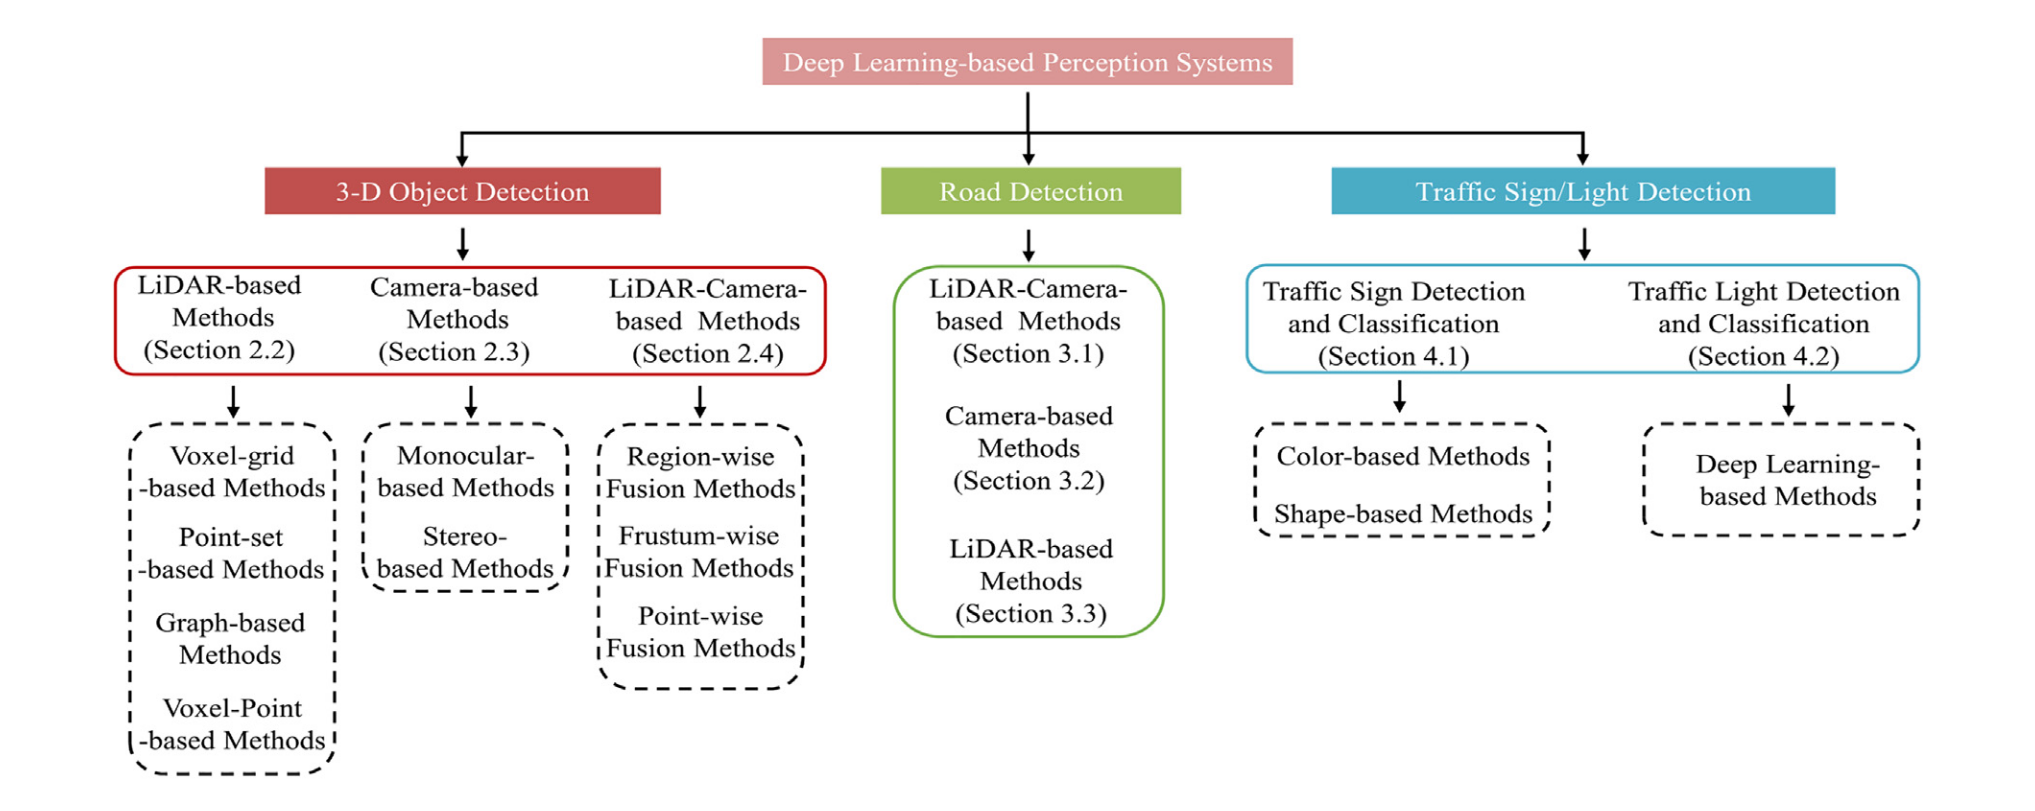
\includegraphics[width=135mm]{figures/learning_based_methods.png}%
  
  \caption{Learning-based perception methods. Source: \cite{learning_based_perception_survey}}%
  \label{fig:learning_based_methods}%
\end{figure}%

Some limitations of learning-based approaches are the need for extensive training data, which can be expensive and time-consuming to collect.
These methods can also struggle to generalize in novel and untrained scenarios, which can be problematic in safety-critical situations where the 
vehicle must make quick decisions based on the perceived environment.

\subsubsection{Deterministic Approaches}

Deterministic approaches use mathematical models to estimate the state of the objects in the scene. 

\paragraph{Optical flow}

Optical flow is a technique used to estimate the motion of objects in the scene by tracking the movement of pixels between consecutive frames.
This method is based on the assumption that the intensity of a pixel remains constant over time, which allows the system to track the movement
of objects based on the changes in pixel intensity \cite{optical_flow_estimation_survey}. Some of the most common optical flow algorithms are the 
Lucas-Kanade method \cite{flow_lucas_kanade} and the Horn-Schunck method \cite{flow_schunck}.

\paragraph{6D Vision}
\label{sec:6D_Vision}

6D vision is a deterministic perception framework that combines stereo vision and motion tracking to estimate the 3D position and velocity
of objects in the scene. Originally introduced by Franke et all \cite{6d_vision_daimler} this method provides a direct
motion estimation without requiring object segmentation. The key principles of 6D Vision are: 

\begin{enumerate}
  \item \textbf{Stereo disparity estimation:} Calculate the disparity between corresponding points in the stereo images to estimate the depth of objects in the scene.
  \item \textbf{Optical flow tracking:} Track the movement of feature points in the scene between consecutive frames.
  \item \textbf{Kalman filtering:} Use Kalman filters to estimate the 6D state vector (position and velocity) of the feature points in the scene.
\end{enumerate}




\section{State of the Art in the FTM}
\label{sec:StateOfTheArtInTheFTM}


The Institute of Automotive Technology (FTM) at the Technical University of Munich has conducted previous research in
the field of environment perception for autonomous and automated vehicles. This section provides an overview of previous work carried 
out at the FTM, particularly regarding the EDGAR research vehicle and the development of deterministic perception systems based on 6D vision.

\subsection{EDGAR Research Vehicle}

The EDGAR (Excellent Driving Garching) research vehicle is a state-of-the-art autonomous driving platform 
developed at FTM \cite{edgar_hardware}. It serves as a testbench for autonomous driving research, including perception, planning, control, 
and sensor fusion. The vehicle is equipped with a multi-sensor setup, comprising:

\begin{enumerate}
  \item \textbf{Stereo and monocular cameras:} For image-based perception and object detection
  \item \textbf{LiDAR sensors:} For 3D mapping and obstacle detection
  \item \textbf{Radar sensors:} For object avoidance and velocity estimation
  \item \textbf{GPS/IMU:} For localization and motion tracking
\end{enumerate}

\begin{figure}[htb]%
  \centering%
  \begin{minipage}{0.3\textwidth}
    \centering
    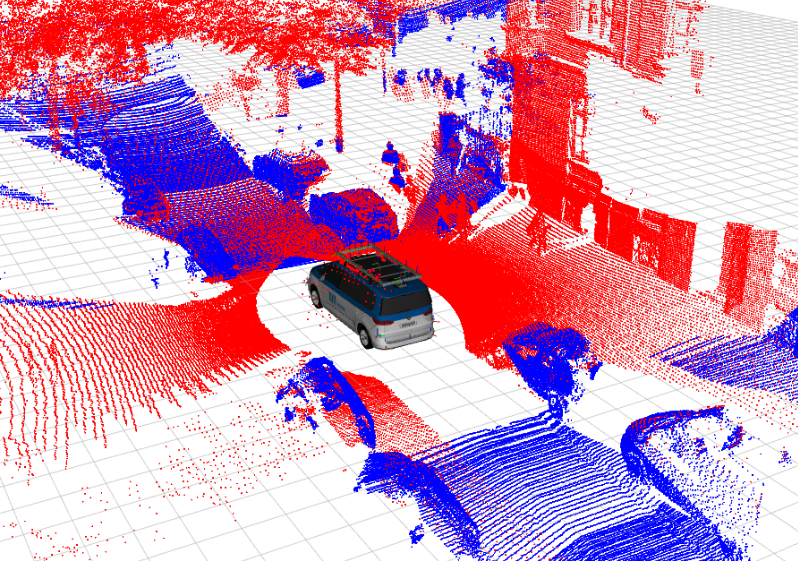
\includegraphics[width=\textwidth]{figures/edgar_3d.png}
  \end{minipage}\hfill
  \begin{minipage}{0.6\textwidth}
    \centering
    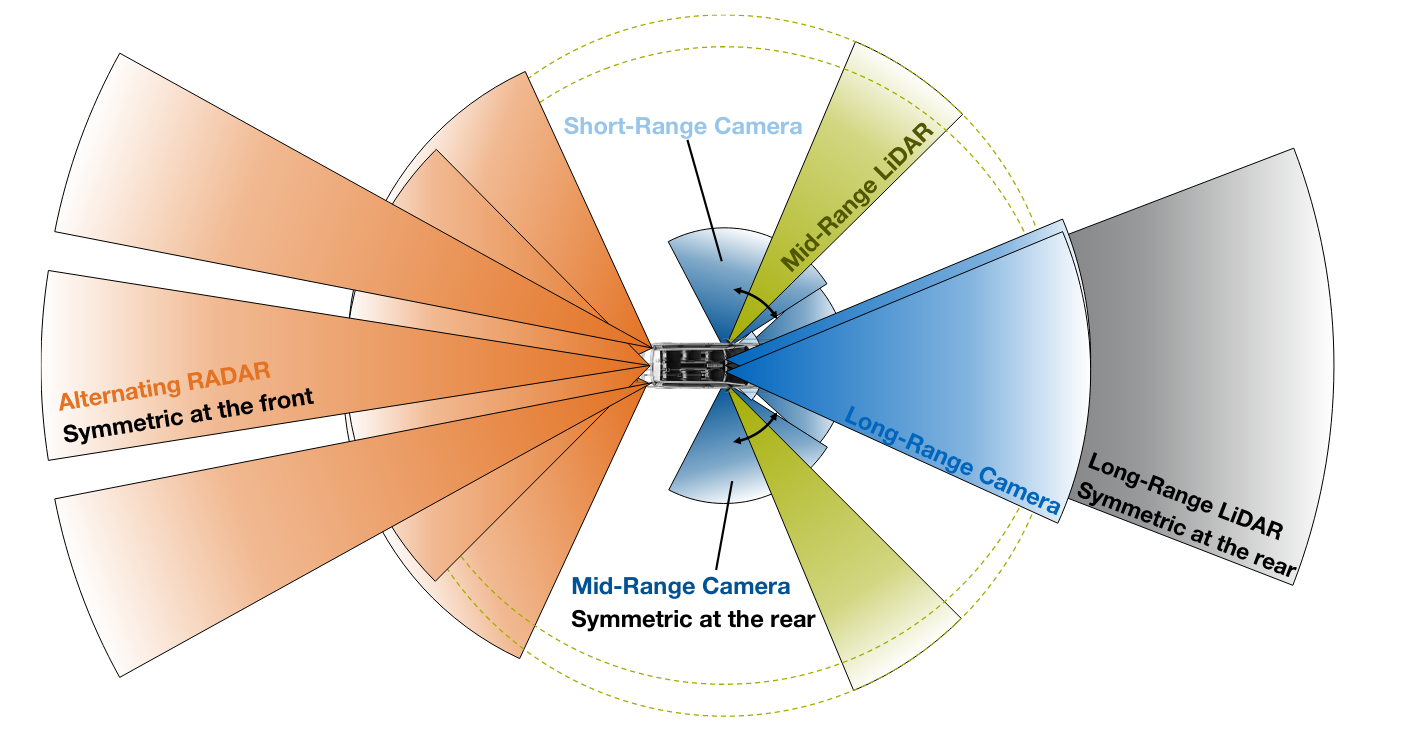
\includegraphics[width=\textwidth]{figures/edgar_sensors.png}
  \end{minipage}
  \caption{EDGAR Vehicle Sensors}
  \label{fig:edgar}%
\end{figure}%



\subsection{Previous Work in the FTM}

This project builds upon previous work conducted at the FTM in the field of environment perception 
for automated vehicles with 6D vision. Some of the key contributions include: 

\begin{enumerate}
  \item \textbf{Objektdetektion und Bewegungsprädiktion mittels eines Stereokamerasystems beim teleoperierten Fahren} \cite{previous_tfm_bauer}: Bauer 
  in his master's thesis developed a deterministic system for object detection based on the 6D vision of Daimler \cite{6d_vision_daimler}. The system 
  was implemented in C++ using the ADTF framework {Automotive Data and Time-Triggered Framework} and was capable of detecting and tracking objects in the vehicle's surroundings 
  with some real time limitations.

  \item \textbf{Weiterentwicklung und echtzeitfähige Umsetzung eines Stereo-Vision-basierten Bewegungsprädiktionssystems für die aktive Sicherheit von teleoperierten Fahrzeugen}
  Some time later in \cite{previous_tfm_gpu_implementation} Rotar continued Bauers work by implementing the system in GPU using CUDA to speed up the computationally intensive tasks.

  \item \textbf{Validation of an Obstacle Detection Approach for Teleoperation of Automated Vehicles:} Finally Pastor \cite{previous_tfm_pastor} started porting the system to ROS1
   to facilitate the integration with other modules in the EDGAR vehicle. The system was implemented without CUDA GPU acceleration
   and was not deployed in the EDGAR vehicle. The system also has some problem with the object detection.
\end{enumerate}

Building upon these previous contributions, this project aims to further improve deterministic perception by 
addressing key limitations found in prior implementations. 
In particular, this work will focus on enhancing computational efficiency, real-time feasibility, 
and system deployment within ROS2. These improvements will be detailed in the next section on objectives.

\section{Stereo camera technology}
\label{sec:StereoCameraTechnology}


\todo{Short review on stereo camera technology.}

\section{Methods for software containerization}
\label{sec:MethodsForSoftwareContainerization}

\todo{Short review on methods for software containerization.}

\section{Requirements for the Thesis}
\label{sec:RequirementsForTheThesis}

\todo{Short review on the requirements for the thesis.}

% =====================================================================
% ================== Methods and Implementation ====================
% ===================================================================
\chapter{Methods and Implementation}
\label{chap:MethodsAndImplementation}

This chapter outlines the methodological and technical approaches that form the foundations
of this project. It begins with a high level architecture of the system, providing insight
into how the different modules interact to enable real-time perception and criticality assessment 
for automated vehicles. 

Following this, each component of the systme is examined in detail, from the underlying algorithms to the
some of the implementation details. Emphasis is placed on the design choices made
to ensure robustness, real-time performance, and modularity.

By decomposing the system into well-defined modules, this architecture enables both scalability and flexibility for experimentation, 
while maintaining consistent performance in real-world conditions. 
It also facilitates further development and seamless integration with other components of the EDGAR vehicle's software stack.

\section{System Architecture}
\label{sec:SystemArchitecture}

The system is conceptually divided into two main pipelines: the perception pipeline and the criticality pipeline. The 
\textbf{perception pipeline} processes raw sensor data captured by the stereo camera to build a dynamic representation of 
the environment and estimating the position and speed vectors of the moving objects. The output of this pipeline is a list
of object in the scene that is later used by the \textbf{criticality pipeline} to compute the criticality score of the detected objects.

\begin{figure}[htb]
  \centering
  \resizebox{1.0\textwidth}{!}{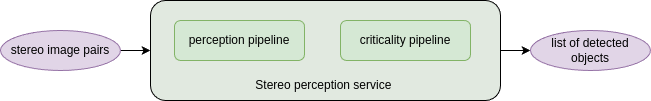
\includegraphics{figures/overall_system.drawio.png}
  \caption{High level overall system}
  \label{fig:system_high_level}
  }
\end{figure}%


\subsection{Perception pipeline}
\label{sec:PerceptionPipeline}  

The perception pipeline will be responsible for detecting moving objects and estimating their position and current velocity. The pipeline consists of several submodules as illustrated in figure \ref{fig:perception_pipeline_high_level}.

\begin{figure}[H]
  \centering
  \resizebox{0.8\textwidth}{!}{

\begin{tikzpicture}[node distance=0.5cm and 2cm, auto]

  % Primera fila: óvalos de entrada (fuera del contenedor, en azul claro)
  \node[draw, ellipse, fill=blue!20] (params) {Left cam. parameters};
  \node[draw, ellipse, fill=blue!20, right=3cm of params] (limg) {Left image};
  \node[draw, ellipse, fill=blue!20, right=3cm of limg] (rimg) {Right image};

  % Segunda fila: rectángulos de cómputo (dentro del contenedor, en verde)
  \node[draw, rectangle, fill=green!20, minimum width=3cm, minimum height=1cm, below=0.7cm of params] (optflow) {Optical flow computation};
  \node[draw, rectangle, fill=green!20, minimum width=3cm, minimum height=1cm, below=0.7cm of limg] (visodom) {Visual odometry computation};
  \node[draw, rectangle, fill=green!20, minimum width=3cm, minimum height=1cm, below=0.7cm of rimg] (depth) {Depth computation};
  
  % Flechas desde la primera fila a la segunda
  \draw[->, thick] (limg) -- (optflow);
  \draw[->, thick] (limg) -- (visodom);
  \draw[->, thick] (params) -- (visodom);
  \draw[->, thick] (limg) -- (depth);
  \draw[->, thick] (params) -- (depth);
  \draw[->, thick] (rimg) -- (depth);

  % Tercera fila: óvalos de salida de los cómputos (dentro del contenedor, en amarillo claro)
  \node[draw, ellipse, fill=yellow!20, below=0.5cm of optflow] (oflow) {Opt. flow image};
  \node[draw, ellipse, fill=yellow!20, below=0.5cm of visodom] (vo) {Visual odometry};
  \node[draw, ellipse, fill=yellow!20, below=0.5cm of depth] (dimage) {Depth image};
  
  % Flechas desde los rectángulos a los óvalos correspondientes
  \draw[->, thick] (optflow) -- (oflow);
  \draw[->, thick] (visodom) -- (vo);
  \draw[->, thick] (depth) -- (dimage);
  
  % Cuarta fila: kalman filter (rectángulo, dentro del contenedor, en verde)
  \node[draw, rectangle, fill=green!20, minimum width=3cm, minimum height=1cm, below=0.5cm of vo] (kalman) {6D Kalman Filter algorithm};
  
  % Flechas desde los óvalos de salida a kalman filter
  \draw[->, thick] (oflow) -- (kalman);
  \draw[->, thick] (vo) -- (kalman);
  \draw[->, thick] (dimage) -- (kalman);
  
  % Flecha curvada desde "left camera parameters" a "kalman filter"
  \draw[->, thick] (params.south east) .. controls +(1.5, -0.5) and +(-1.5, 0.5) .. (kalman.north west);
  
  % Quinta fila: óvalo "6d image" (dentro del contenedor, en amarillo claro)
  \node[draw, ellipse, fill=yellow!20, below=0.5cm of kalman] (sixd) {6D image};
  \draw[->, thick] (kalman) -- (sixd);
  
  % Sexta fila: rectángulo "Clustering" (dentro del contenedor, en verde)
  \node[draw, rectangle, fill=green!20, minimum width=3cm, minimum height=1cm, below=0.5cm of sixd] (clustering) {Clustering algorithm};
  \draw[->, thick] (sixd) -- (clustering);
  
  % Detected objects: óvalo fuera del contenedor (en azul claro), ubicado abajo
  \node[draw, ellipse, fill=blue!20, below=0.7cm of clustering] (detected) {Detected objects};
  \draw[->, thick] (clustering) -- (detected);
  
  % Contenedor: agrupa los nodos del pipeline (excepto la primera fila y "detected objects")
  \node[draw, dotted, inner sep=0.5cm, fit=(optflow) (visodom) (depth) (oflow) (vo) (dimage) (kalman) (sixd) (clustering)] (perception) {};
  \node[anchor=south east, inner sep=2mm] at (perception.south east) {perception pipeline};
  
\end{tikzpicture}}
  \caption{High level perception pipeline}
  \label{fig:perception_pipeline_high_level}
\end{figure}%

As shown in the figure, the perception pipeline comprises the following core modules: 

\todo{Search source of sgm algorithm}

\begin{enumerate}
  \item \textbf{Optical flow computation:} Calculates a dense optical flow field from the left image sequence
  using the Farneback algorithm.

  \item \textbf{Visual odometry:} Estimates the ego-motion of the vehicle using stereo image sequences
  \item \textbf{Depth computation:}  Computes a dense depth image from the stereo image pair using a semi-global
  matching (SGM) algorithm.
  \item \textbf{Kalman filter:}  Central module of the perception pipeline. It uses depth and optical flow data to
  estimate the 6D state (position and velocity) of a sparse set of points over time.
  \item \textbf{Object detection:} Applies a clustering algorithm (DBSCAN) to group similar 6D points into
  detected objects.
\end{enumerate}

\subsection{Criticallity pipeline}
\label{sec:CriticallityPipeline}

The criticality pipeline (Figure~\ref{fig:cp_high_level}) assesses the risk posed by each detected
object. Based on the output of the perception pipeline and the current trajectory of the ego-vehicle,
it computes criticality metrics such as the Time-to-Collision (TTC) \cite{cricitality_metrics}. These
metrics serve as indicators of potential hazards in the environment.


\begin{figure}[h]
  \centering
  \resizebox{0.2\textwidth}{!}{\begin{tikzpicture}[node distance=1.5cm, auto]

  % Nodo de entrada (fuera del contenedor)
  \node[draw, ellipse, fill=blue!20] (detected) {detected objects};
  
  % Nodo del algoritmo (dentro del contenedor)
  \node[draw, rectangle, fill=green!20, minimum width=3cm, minimum height=1cm, below=of detected] (algo) {criticality algorithm};
  
  % Nodo de salida (fuera del contenedor)
  \node[draw, ellipse, fill=blue!20, below=of algo] (metrics) {criticality metrics};
  
  % Flechas de conexión
  \draw[->, thick] (detected) -- (algo);
  \draw[->, thick] (algo) -- (metrics);
  
  % Contenedor punteado que engloba solo el algoritmo
  \node[draw, dotted, inner sep=0.5cm, fit=(algo)] (pipeline) {};
  \node[anchor=south east, inner sep=1mm] at (pipeline.south east) {      criticality pipe.};
  
\end{tikzpicture}}
  \caption{High level criticality pipeline}
  \label{fig:cp_high_level}
\end{figure}%

\subsection{Repository structure}
\label{sec:RepositoryStructure}

The project is implemented as a monorepo, consolidating all system components into a single, unified 
repository to simplify development, integration, and deployment.

The repository is structured into three main directories:

\begin{itemize}
  \item \textbf{src:} Contains all ROS 2 source code. It is further divided into:
  \begin{itemize}
    \item \textbf{launch\_packages}: Includes ROS 2 launch files used to start multiple components together.
    \item \textbf{perception\_pipeline}: Contains the core modules of the perception pipeline, including
    \textbf{camera\_info\_publisher}, \textbf{stereo\_computation}, \textbf{optical\_flow\_computation}, 
    \textbf{kalman\_filter}, and \textbf{object\_detector}.
    \item \textbf{criticality\_pipeline}: Contains the \textbf{ttc\_calculator} package responsible for computing
    Time-to-Collision and other criticality metrics.
    \item \textbf{utils}: Provides auxiliary packages and shared message definitions in \textbf{stereo\_perception\_msgs}.
  \end{itemize}
  
  \item \textbf{scripts:} Includes helper bash scripts and Dockerfiles used to build, run, and deploy the system.

  \item \textbf{config/dds:} Contains configuration files related to middleware settings such as DDS profiles.
\end{itemize}

An overview of this structure is shown in Figure~\ref{fig:repo_structure}.

\begin{figure}[H]
  \centering
  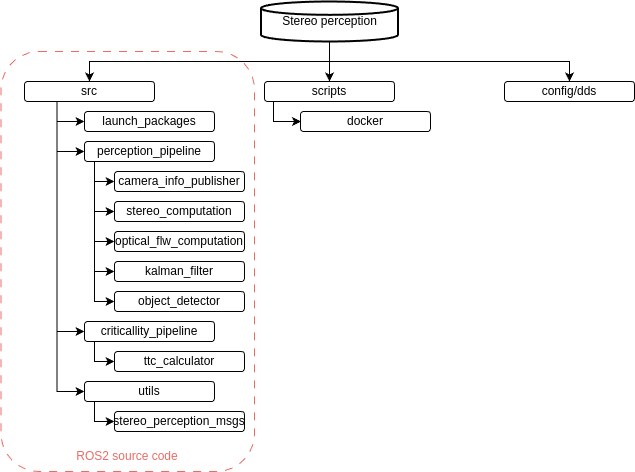
\includegraphics[width=0.85\textwidth]{figures/repository_structure.drawio.png}
  \caption{Overview of the repository structure}
  \label{fig:repo_structure}
\end{figure}


\subsection{Containerization}
\label{sec:Containerization}

Docker is a platform for developing, shipping, and running applications in lightweight, isolated
environments called containers. Containers package the application code together with its
dependencies and runtime, ensuring consistent behavior across different systems and deployment
contexts.

To ensure reproducibility, portability, and streamlined deployment, the entire system is encapsulated
within a single Docker container. This design choice is driven by both functional and performance
considerations.

Firstly, the system is architected as a unified perception service that processes synchronized stereo
camera inputs to produce a list of detected objects along with their associated criticality scores.
Given the tight coupling and interdependencies among the modules, segregating components into
multiple containers would introduce unnecessary inter-process communication overhead.

Secondly, employing a single container mitigates latency introduced by serialization and network
layers between containers. This is particularly crucial in real-time systems, where maintaining low
processing latency is imperative. Running all modules in the same memory space allows for efficient
data exchange and eliminates potential bottlenecks associated with inter-container messaging.

This containerization strategy also simplifies integration with the research platform, facilitating
easier deployment, logging, and testing within a controlled and reproducible environment.

\todo{Explain how it was built: OpenCV, CUDA, ROS2, etc.}


\newpage
\section{Perception pipeline: Stereo image computation}
\label{sec:PerceptionPipelineStereoImageComputation}

The stereo image computation module is responsible for generating a dense depth map from a pair of
rectified stereo images and its calibration parameters. This component is particularly relevant when 
working with datasets or sensors that provide raw stereo image pairs but no precomputed depth information. Although this
module is not used in the final deployment of the system on the EDGAR research vehicle, since its
stereo camera setup provides depth images directly—it plays a crucial role in training, testing, and
benchmarking the system using external datasets. It can also be used in the future to integrate other
stereo camera sets that do not provide depth images.

\subsection{Mathematical Background: Pinhole Camera Model and Disparity}

In stereo vision, depth estimation relies on the triangulation of corresponding points in a pair of 
images captured from slightly different viewpoints. The pinhole camera model (figure: \ref{fig:pinhole_camera_model}) is commonly used to describe the 
relationship between 3D world coordinates and 2D image coordinates. In this model, a 3D point $\mathbf{P} = (X, Y, Z)$ 
is projected onto the image plane as a 2D point $\mathbf{p} = (x, y)$ using the camera's intrinsic parameters (\cite{pin_hole_camera_model}).
These parameters include the focal length $f$ and the principal point $(c_x, c_y)$, which define the camera's optical center and field of view.

\begin{figure}[H]
  \centering
  \resizebox{0.4\textwidth}{!}{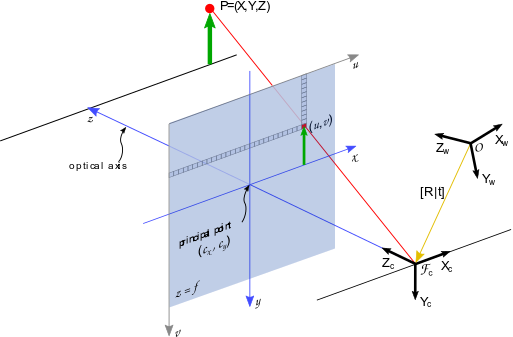
\includegraphics{figures/pinhole_camera.png}}
  \caption{Pinhole camera model. Source: Nvidia \label{fig:pinhole_camera_model}}
\end{figure}%

The relationship between the 3D point and its 2D projection is given by:

\begin{equation}
  \begin{bmatrix}
  x \\
  y \\
  1
  \end{bmatrix}
  = 
  \frac{1}{Z}
  \begin{bmatrix}
  f_x & 0 & c_x \\
  0 & f_y & c_y \\
  0 & 0 & 1
  \end{bmatrix}
  \begin{bmatrix}
  X \\
  Y \\
  Z
  \end{bmatrix}
\end{equation}

where $f_x$ and $f_y$ are the focal lengths in pixels, and $(c_x, c_y)$ is the principal point.

In a typical stereo setup, the two cameras are displaced horizontally along the x-axis, with their 
optical axes kept parallel. This physical separation between the cameras is known as the 
\textbf{baseline} $B$, as seen in the figure \ref{fig:stereo_camera_setup_disparity} left. The baseline is a key parameter in stereo vision, as it directly influences 
the triangulation accuracy: a larger baseline improves depth resolution, especially for distant 
objects, but also increases the difficulty of finding correct correspondences due to greater viewpoint differences.

\begin{figure}[H]
  \centering
  \begin{minipage}{0.343\textwidth}
    \centering
    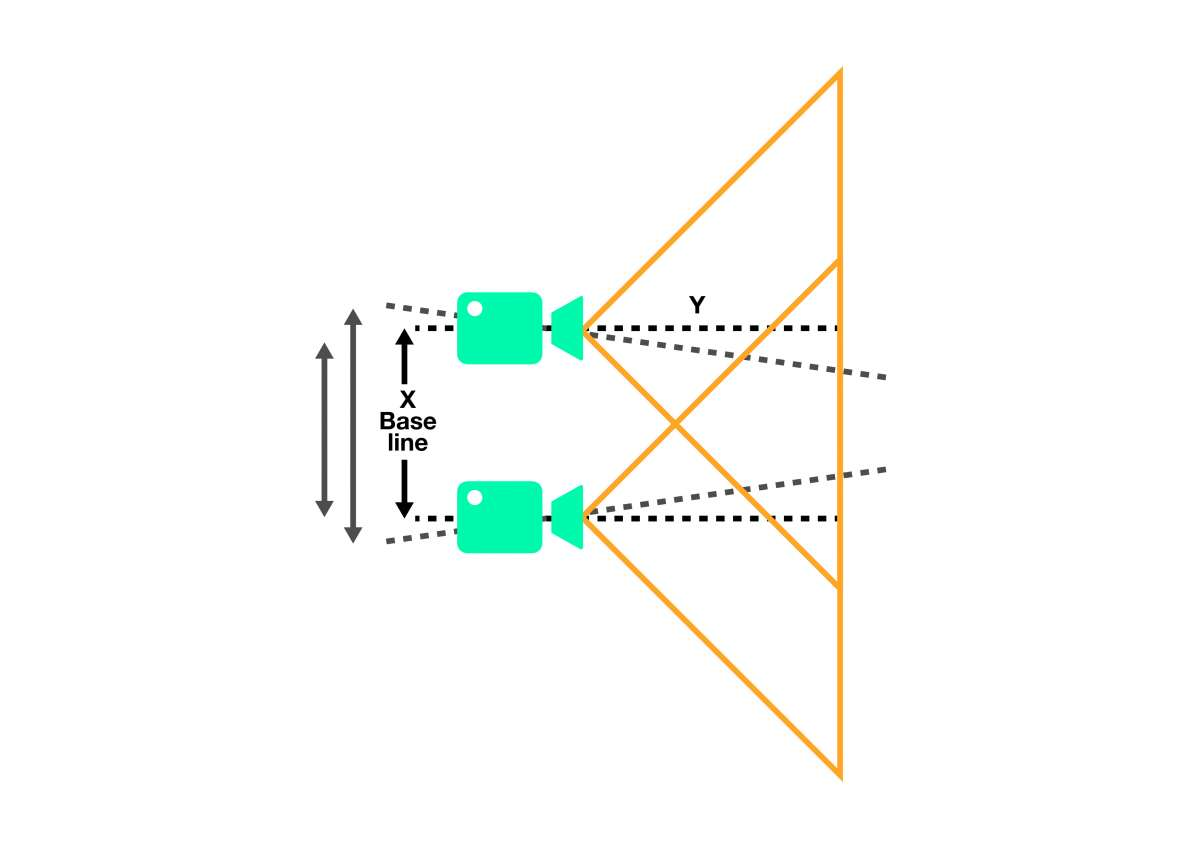
\includegraphics[width=\textwidth]{figures/framos_stereo_setup.jpg}
  \end{minipage}
  \hfill
  \begin{minipage}{0.62\textwidth}
    \centering
    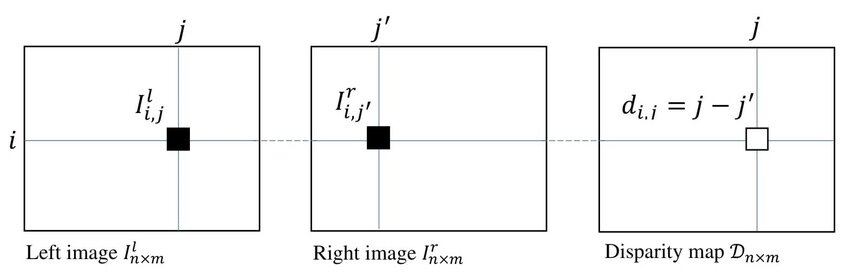
\includegraphics[width=\textwidth]{figures/disparity_map.png}
  \end{minipage}
 \caption{Stereo camera setup (left) and disparity concept (right). Source: Framos, \cite{disp_map_figure}.}
\label{fig:stereo_camera_setup_disparity}
\end{figure}


Thanks to this horizontal arrangement, the correspondence search simplifies to a one-dimensional 
problem along the image rows. After rectification, corresponding points between the two images lie 
along the same horizontal line (epipolar line), and the \textbf{disparity} $d$ (figure \ref{fig:stereo_camera_setup_disparity} right) between corresponding 
points is defined as:

\begin{equation}
  d = x_{\text{left}} - x_{\text{right}}
\end{equation}
  
Disparity is inversely proportional to the depth of the observed point. The relation between disparity 
and depth $Z$ is given by:
  
\begin{equation}
Z = \frac{f \cdot B}{d}
\end{equation}

\subsection{Stereo Matching Algorithms}

Stereo matching algorithms are responsible for computing the disparity map between a pair of 
rectified stereo images. Given that disparity directly relates to depth, these algorithms are a 
critical component of the stereo vision pipeline. Their main task is to find, for each pixel in the 
left image, the corresponding pixel in the right image along the same horizontal line.

Several approaches exist to solve this correspondence problem, each with different trade-offs 
between computational complexity, robustness, and accuracy. Some of the most common implemented stereo
matching algorithms include:

\begin{itemize}
  \item \textbf{Block Matching (BM):} A local method that compares fixed-size blocks between the left and right images. While computationally efficient, it often struggles with textureless regions and depth discontinuities (\cite{disparity_block_matching}). 
  \item \textbf{Semi-Global Matching (SGM):} An algorithm that balances accuracy and computational efficiency by aggregating matching costs along multiple paths through the image (\cite{disparity_sgm}).
\end{itemize}

Comparative studies (\cite{disparity_survey}) have shown that SGM offers a good trade-off between accuracy and performance, making it suitable for real-time applications where both speed and quality are essential.


\subsection{Semi-Global Matching (SGM)}
\label{sec:SGM}

Semi-Global Matching (SGM) is a stereo matching algorithm that offers a compromise between the 
accuracy of global optimization methods and the computational efficiency of local methods. It was first
introduced by Hirschmüller~\cite{disparity_sgm} and has become widely implemented in real-time 
applications.

The underlying principle in SGM is to minimize a global energy function that imposes continuity in the
disparity map, having strong depth discontinuities along object boundaries. The energy function $E(D)$
for a disparity map $D$ is defined as:

\begin{equation}
E(D) = \sum_{\mathbf{p}} \left( C(\mathbf{p}, D_{\mathbf{p}}) + \sum_{\mathbf{q} \in \mathcal{N}_{\mathbf{p}}} 
P_1 \cdot \delta\left( |D_{\mathbf{p}} - D_{\mathbf{q}}| = 1 \right) + P_2 \cdot \delta\left( |D_{\mathbf{p}} - D_{\mathbf{q}}| > 1 \right) \right)
\end{equation}

where:
\begin{itemize}
  \item $C(\mathbf{p}, D_{\mathbf{p}})$ is the matching cost at pixel $\mathbf{p}$ for disparity $D_{\mathbf{p}}$.
  \item $\mathcal{N}_{\mathbf{p}}$ denotes the set of neighboring pixels.
  \item $P_1$ and $P_2$ are penalty terms for disparity changes of 1 and greater than 1, respectively.
  \item $\delta$ is the Kronecker delta function.
\end{itemize}

The algorithm operates in two main steps:

\textbf{1. Cost computation:}  
For each possible disparity, a matching cost calculation happens between the left picture plus 
the right picture at each pixel. This calculation uses methods like the Sum of Absolute Differences 
or measurements that use census transform.

\textbf{2. Cost aggregation:}  
SGM does not do a full 2D global optimization. That process demands a lot of computation, so it 
is not practical for systems that need to run in real time. SGM comes close to global reasoning when 
it combines costs along several 1D paths. Costs are put together along either 4 or 8 directions from
each pixel. A dynamic programming method finds the lowest local cost in each direction. 
It also adds penalties for significant changes in disparity.

Once the cost values are added together from all directions, the disparity picked for each pixel is the one that has the lowest combined cost.


This balance between accuracy and computational efficiency makes SGM highly attractive for embedded 
and real-time applications. 

\subsection{ROS2 Implementation}
\label{sec:ROS2Implementation}

The SGM algorithm has been integrated into the pipeline with a dedicated ROS2 package called 
\texttt{stereo\_computation}.It contains a node that subscribes to three topics: the rectified left and right 
camera images, and the camera info topic of the left camera. 
After receiving synchronized input, the node computes both the disparity map and the depth map, 
which are then published on two separate ROS2 topics for downstream processing.

The stereo matching algorithm was implemented using the OpenCV library. In particular, the 
\texttt{cv::cuda::StereoSGM} class was chosen to compute the disparity map. This class offers a 
CUDA-accelerated version of the Semi-Global Matching algorithm, enabling the computations to be 
performed directly on the GPU. Taking advantage of GPU acceleration is crucial to meet the real-time 
performance requirements of the perception pipeline.

The OpenCV implementation of SGM is highly optimized and designed to exploit the parallel 
architecture of modern GPUs, significantly reducing the runtime compared to CPU-based methods. 
After computing the disparity map, the depth map is generated by applying the classical 
pinhole camera equation:

\begin{equation}
Z = \frac{f \cdot B}{d}
\end{equation}

where $Z$ is the depth value, $f$ is the focal length of the camera, $B$ is the baseline distance 
between the two cameras, and $d$ is the disparity.

This node architecture ensures modularity within the perception pipeline and allows easy 
integration with other modules, such as the Kalman filtering and object detection components. 
Furthermore, by publishing both the disparity and depth images, the system maintains flexibility 
for future extensions or algorithm improvements that may require direct access to raw disparity data.

To make the tuning and implementation easier, the following ROS2 parameters were added to the node:

\begin{table}[H]
  \begin{tabular}{|l|l|}
  \hline
  ROS2 parameter               & Definition                                                                    \\ \hline
  in\_left\_image\_topic       & Topic name for the left input grayscale image                                 \\ \hline
  in\_right\_image\_topic      & Topic name for the right input grayscale image                                \\ \hline
  in\_camera\_info\_topic      & Topic name for the camera calibration information                             \\ \hline
  out\_depth\_image\_topic     & Output topic for the computed depth image                                     \\ \hline
  out\_disparity\_image\_topic & Output topic for the computed disparity image                                 \\ \hline
  min\_disparity               & Minimum disparity to consider for the disparity calculation                   \\ \hline
  num\_disparities             & Number of disparities (disparity range) to compute                            \\ \hline
  P1                           & Control parameter for the SGM algorithm (penalty for small disparity changes) \\ \hline
  P2                           & Control parameter for the SGM algorithm (penalty for small disparity changes) \\ \hline
  uniqueness\_ratio            & Threshold for uniqueness of matching points (higher means stricter matching)  \\ \hline
  speckle\_window\_size        & Size of the window used for speckle filtering                                 \\ \hline
  speckle\_range               & Maximum disparity range for speckle filtering                                 \\ \hline
  pre\_filter\_cap             & Pre-filtering parameter for the image to improve disparity computation        \\ \hline
  use\_sim\_time               & Flag to use simulation time instead of system time                            \\ \hline
  \end{tabular}
  \end{table}
and the node can be added to a launch file as seen in the following example:

\begin{lstlisting}[language=FTMpython,style=PythonStyleFTM,caption={Stereo computation launch},label={code:scl}]
  launch_ros.actions.Node(
              package='stereo_computation', 
              executable='stereo_computation_node',
              output='screen',
              parameters=[
                {"in_left_image_topic": input_gray_left_topic},
                {"in_right_image_topic": input_gray_right_topic},
                {"in_camera_info_topic": input_camera_info_topic},
                {"out_depth_image_topic": "perception_pipeline/depth_image"},
                {"out_disparity_image_topic": "perception_pipeline/disparity"},
                {"min_disparity": 0},
                {"num_disparities": 256},
                {"P1": 30},
                {"P2": 200},
                {"uniqueness_ratio": 15},
                {"speckle_window_size": 50},
                {"speckle_range": 2},
                {"pre_filter_cap": 31},
                {"use_sim_time": use_sim_time}
                ],
            ),
\end{lstlisting}%

\newpage
\section{Perception pipeline: Optical flow computation}
\label{sec:PerceptionPipelineOpticalFlowComputation}

This section describes the optical flow computation module within the perception pipeline.
This module is responsible for estimating the relative motion of the pixels of the image between
two consecutive frames.

\subsection{Optical flow concept}
\label{sec:OpticalFlowConcept}
The concept of Optical Flow, first introduced by James Gibson in the 1950s (\cite{optical_flow_concept}) 
refers to the displacements of intensity patterns.  In our case it represents the relative motion 
of the pixels between two consequtive frames of a video stream. The output is  a 2D vector field where 
each vector describes the position of a pixel or a small region in the current frame relative to its 
position in the previous frame.

This module is crucial for estimating the information of how the pixels in the image are moving, which is
one of the essential inputs to the Kalman Filter stage. 

\begin{figure}[H]
  \centering
  \resizebox{0.6\textwidth}{!}{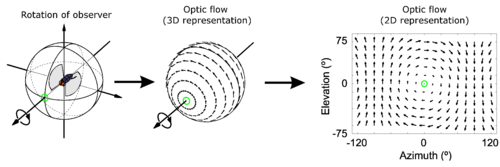
\includegraphics{figures/opt_flw_concept.png}}
  \caption{Optical flow}
  \label{fig:optical_flow_concept}
\end{figure}%

Optical flow estimation relies on the assumotion that the brightness of a pixel remains constant
over time \cite{optical_flow_review_2025,optical_flow_computation_survey}, which allows the system to track the movement of objects based on the changes in pixel
intensity.  Mathematically, this assumption leads to the optical flow constraint equation:
\begin{equation}
  I_x u + I_y v + I_t = 0
\end{equation}  

Where: 

\begin{itemize}
  \item $I_x$ and $I_y$ are the spatial gradients of the image intensity in the x and y directions.
  \item $I_t$ is the temporal gradient of the image intensity (the difference between two consecutive frames).
  \item $u$ and $v$ are the optical flow components in the x and y directions.
\end{itemize}

Since there is one equation and two unknowns, the optical flow constraint equation is underdetermined.
To solve this problem, additional constraints or assumptions are needed, leading to different 
optical flow algorithms.

\subsection{Optical flow algorithms}
\label{sec:OpticalFlowAlgorithms}

Optical flow methods can be classified into two main categories: sparse and dense optical flow.

\textbf{Sparse optical flow} methods focus on estimating motion vectors at a discrete set of 
key points in the image. These points are typically features such as corners or edges that 
can be tracked reliably across frames. In contrast, \textbf{dense optical flow} methods aim 
to estimate a motion vector for every pixel in the image, providing a complete 2D 
displacement field.

\begin{figure}[H]
  \centering
  \resizebox{0.8\textwidth}{!}{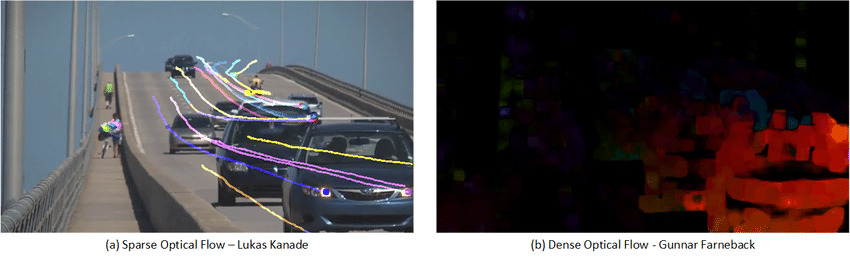
\includegraphics{figures/sparse_vs_coarse_opt_flw.jpg}}
  \caption{Sparse vs dense optical flow. Source: \cite{figure_sparse_vs_dense_opf_flw}}
  \label{fig:sparse_vs_dense_optical_flow}
\end{figure}%

Recently, deep learning-based methods have gained popularity and demonstrated impressive
performance for optical flow estimation. Models such as FlowNet~\cite{opt_flw_flownet} and
RAFT~\cite{opt_flw_raft} leverage convolutional neural networks (CNNs) to learn spatial and temporal
features from large datasets, enabling them to predict optical flow fields with high accuracy. However,
these methods often require significant computational resources and may suffer from poor
generalization to unseen environments.

For these reasons, and due to the necessity of robustness and real-time performance, this work focuses
on traditional deterministic optical flow algorithms. These classical methods also offer the advantage
of being widely implemented and optimized in existing libraries, which significantly accelerates
development and integration time.

Some of the most common optical flow algorithms include \cite{optical_flow_estimation_survey,opt_flw_old_survey}: 

\begin{itemize}
  \item \textbf{Lucas-Kanade method~\cite{flow_lucas_kanade}:}
  
  Introduces in 1981 by Lucas and Kanade, this os a sparse optical flow method based on the assumption
  of constant optical flow within a small local neighborhood. It solves the optical flow constraint
  equation using a least-squares approach. This method is simple and computationally efficient, but it is 
  sensitive to large motions and requires good texture in the tracked regions.

  \item \textbf{Horn-Schunck method~\cite{opt_flw_schunck}:}
  
  Proposed by Horn and Schunck, this method computed dense optical flow by introducing a global smoothness
  constraint. It formulates flow estimation as the minimization of an enegy function that combines the 
  brightness constancy constraint and a smoothness term. While robust to moredate noise and capable of estimating
  full dense flow, the method can oversmooth motion boundaries and struggles with large displacements.

  \item \textbf{TV-L1 method~\cite{opt_flw_tv_l1}:} 
  
  This approach refines the variational method of Horn and Schunck by introducing a total variation (TV) 
  regularization term and an L1 norm for the data term. The resulting algorithm is more robust and was 
  implemented in the previous work of Bauer \cite{previous_tfm_bauer}. Nevertheless, it is computationally
  expensive and may not be the best choice for real-time applications.

  \item \textbf{Farneback method~\cite{opf_flw_farneback}:}
  Farneback introduced a dense optical flow method based on local polynomial expansions. The idea is to 
  approximate the neighborhood of each pixel ith a quadratic polynomial and then estimate how the polynomials
  change between frames. 

  This method offers a good trade-off between accuracy and computational efficiency. When accelerated using
  GPUs (e.g. via OpenCV CUDA modules), it can achieve real-time performance even on high-resolution images.
\end{itemize}

In this work, the Farneback method has been selected due to its computational efficiency, robustness for medium-range motions,
and the availability of an optimized CUDA implementation.

\subsection{Farneback algorithm}
\label{sec:FarnebackAlgorithm}

The Farneback optical flow method is a dense flow estimation algorithm based on polynomial
expansion of local image neighborhoods. Its core idea is to approximate the intensity variation in
a small image region using a quadratic polynomial, and then infer the motion between frames by
analyzing how these polynomials deform over time.

The first step is to approximate the image intensity function $I(x, y)$ in a local neighborhood
using a second-order Taylor expansion:
\begin{equation}
I(x, y) \approx x^T A x + b^T x + c
\end{equation}
where:
\begin{itemize}
  \item $x = (x, y)^T$ represents the spatial coordinates,
  \item $A$ is a symmetric $2\times2$ matrix encoding the second-order spatial derivatives,
  \item $b$ is a $2\times1$ vector representing the first-order spatial derivatives,
  \item $c$ is a scalar term corresponding to the local intensity offset.
\end{itemize}

This local polynomial approximation can be efficiently computed over the entire image using
Gaussian-weighted least squares fitting, a process known as polynomial expansion.

When the scene undergoes a pure translation $d = (d_x, d_y)^T$ between two consecutive frames,
the transformed intensity function $I'(x)$ can be related to the original by:
\begin{equation}
I'(x) = I(x - d)
\end{equation}

Substituting the polynomial approximation yields:
\begin{equation}
I'(x) \approx (x - d)^T A (x - d) + b^T (x - d) + c
\end{equation}

Expanding the right-hand side leads to:
\begin{equation}
I'(x) \approx x^T A x + (b - 2Ad)^T x + (d^T A d - b^T d + c)
\end{equation}

Comparing terms, we observe that:
\begin{align}
A' &= A \\
  b' &= b - 2Ad \\
  c' &= d^T A d - b^T d + c
\end{align}
where $A'$ and $b'$ represent the new polynomial coefficients after displacement.

Thus, the displacement $d$ can be estimated by solving the linear system:
\begin{equation}
2A d = b - b'
\end{equation}
assuming that $A$ is non-singular and well-conditioned.

In practice, direct estimation is complicated by noise, local deformations, and the limited validity of
polynomial approximations. To address these issues, the following refinements are applied:
\begin{itemize}
  \item Estimate the displacement over a local window using Gaussian weighting to prioritize central pixels.
  \item Aggregate local estimates using weighted least squares to improve robustness against noise.
  \item Employ a multi-scale coarse-to-fine pyramid approach to capture both small and large displacements effectively.
\end{itemize}

\subsubsection*{Coarse-to-fine pyramid approach}

Large displacements between frames can cause local matching failures if only a single resolution
is used. To handle this, the Farneback method employs a coarse-to-fine multi-scale pyramid strategy
\cite{opt_flw_coarse_to_fine}.

\begin{figure}[H]
  \centering
  \resizebox{0.8\textwidth}{!}{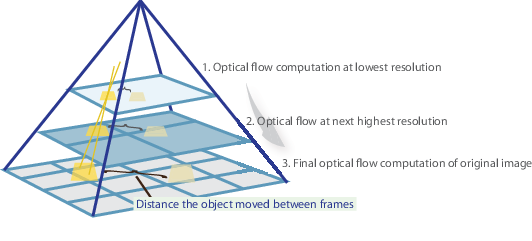
\includegraphics{figures/pyramid.png}}
  \caption{Coarse-to-fine pyramid approach. Source: Matlab}
  \label{fig:opf_flw_pyramid}
\end{figure}%

In the pyramid approach:
\begin{itemize}
  \item The original images are repeatedly downsampled by a scaling factor (typically 0.5), producing
  several lower-resolution versions.
  \item Optical flow is first estimated at the coarsest (smallest) scale, where large motions appear reduced
  and easier to estimate.
  \item The initial flow estimate is then propagated to the next finer scale, where it is refined using the
  higher-resolution image data.
  \item This process continues until the finest scale (the original resolution) is reached, producing a dense
  and detailed optical flow field.
\end{itemize}

The pyramid-based coarse-to-fine strategy is crucial for ensuring that large motions do not overwhelm the local
polynomial approximation, maintaining both the accuracy and robustness of the Farneback method.

This hierarchical refinement significantly enhances the capability of the algorithm to deal with large
inter-frame displacements, dynamic scenes, and varying object velocities.

\subsection{Implementation}
\label{sec:ImplementationOpticalFlow}

This algorithm has been implemented in a ROS2 package called \texttt{optical\_flow\_computation}.
This package contains a node responsible for computing the optical flow between two consecutive images.
The node subscribes to two topics: the first for the left image and the second for the right image.
Once it receives both images, it computes the optical flow and publishes the result on an output topic.

Regarding the algorithm implementation, the \texttt{cv::cuda::FarnebackOpticalFlow} class from OpenCV
was used. This class provides a CUDA-accelerated version of the Farneback algorithm, allowing computations
to be performed directly on the GPU. The OpenCV implementation of the Farneback algorithm is highly optimized
and designed to leverage the parallel architecture of modern GPUs, significantly reducing execution time compared
to CPU-based methods. This class is included in the header \texttt{opencv2/cudaoptflow.hpp}, which generally
requires manually building OpenCV with CUDA support.

\begin{figure}[H]
  \centering
  \resizebox{0.2\textwidth}{!}{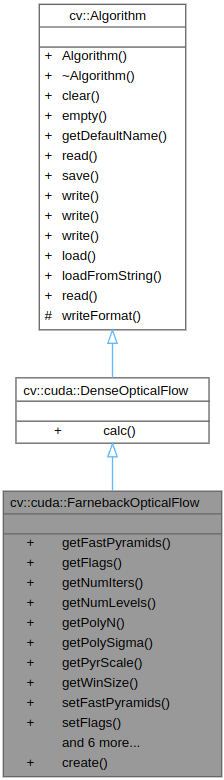
\includegraphics{figures/cuda_opt_flw.png}}
  \caption{CUDA Farneback class. Source: OpenCV}
  \label{fig:opf_flw_cuda}
\end{figure}%

To facilitate tuning and configuration, the following ROS2 parameters were added to the node:

\begin{table}[H]
  \begin{tabular}{|l|l|}
  \hline
  ROS2 parameter       & Definition \\ \hline
  image\_topic         & Input topic name for raw RGB images used in optical flow estimation \\ \hline
  optical\_flow\_topic & Output topic name where the computed optical flow is published \\ \hline
  pyr\_scale           & Scaling factor between pyramid levels \\ \hline
  levels               & Number of pyramid layers, including the original image \\ \hline
  winsize              & Averaging window size for smoothing derivatives; larger values improve robustness but may oversmooth motion boundaries \\ \hline
  iterations           & Number of iterations at each pyramid level; higher values improve convergence in complex motion areas \\ \hline
  poly\_n              & Size of the pixel neighborhood used for polynomial expansion \\ \hline
  poly\_sigma          & Standard deviation of the Gaussian used to smooth derivatives before polynomial expansion \\ \hline
  flags                & Operation flags passed to the Farneback function \\ \hline
  use\_sim\_time       & Boolean indicating whether to use simulation time (\texttt{/clock}) instead of system time \\ \hline
  \end{tabular}
  \caption{ROS2 parameters for the optical flow computation node}
  \label{tab:opf_flw_ros2_params}
\end{table}

The node can be added to a launch file as shown in the following example:

\begin{lstlisting}[language=FTMpython,style=PythonStyleFTM,caption={Optical flow computation launch},label={code:opf_flw_launch}]
launch_ros.actions.Node(
            package='optical_flow_computation', 
            executable='optical_flow_node',
            output='screen',
            parameters=[
              {"image_topic": input_gray_left_topic},
              {"optical_flow_topic": "perception_pipeline/optical_flow"},
              {"pyr_scale": 0.5},
              {"levels": 3},
              {"winsize": 15},
              {"iterations": 3},
              {"poly_n": 5},
              {"poly_sigma": 1.2},
              {"flags": 0},
              {"use_sim_time": use_sim_time}
              ],
          ),
\end{lstlisting}%

The output image is published on the topic \texttt{/perception\_pipeline/optical\_flow}. This image is published
as a \texttt{sensor\_msgs/Image} message with a \texttt{32FC2} encoding format, representing a 32-bit floating-point
optical flow image with two channels. The first channel corresponds to the displacement along the x-axis,
and the second channel corresponds to the displacement along the y-axis.

In addition to the flow image, two debug images are published on the \texttt{/debug} topic to facilitate debugging
and result visualization. One debug image shows the original image with optical flow vectors superimposed,
and the other displays an RGB image where the intensity represents the magnitude of the optical flow vector
and the color represents its direction.

\begin{figure}[H]%
  \centering%
  \begin{minipage}{0.5\textwidth}
    \centering
    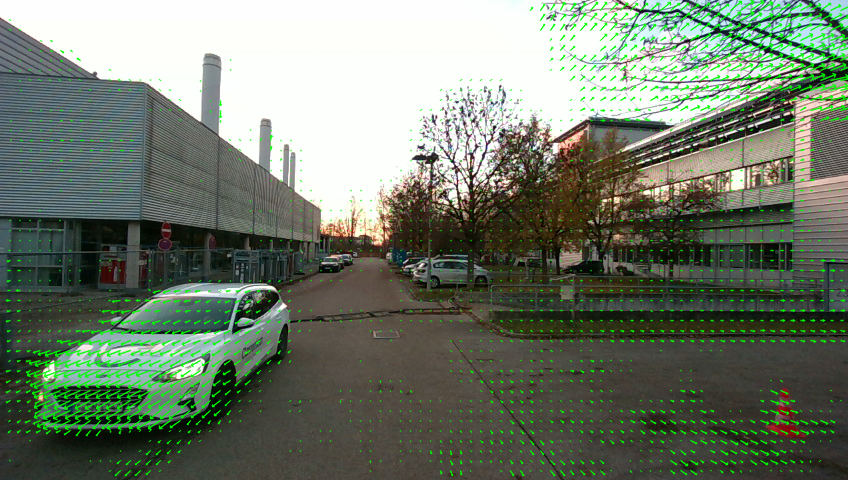
\includegraphics[width=\textwidth]{figures/debug_arrows.png}
  \end{minipage}\hfill
  \begin{minipage}{0.5\textwidth}
    \centering
    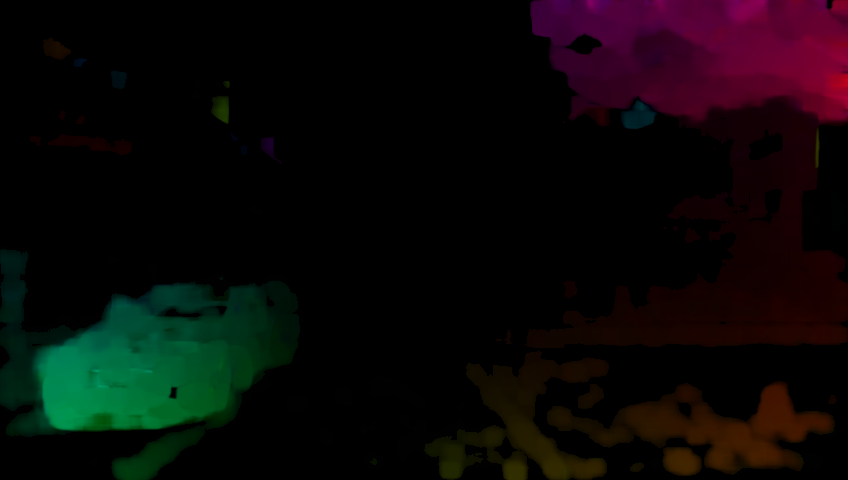
\includegraphics[width=\textwidth]{figures/debug_colored_image.png}
  \end{minipage}
  \caption{Optical flow debug images. Left: Optical flow vectors superimposed on the original image. Right: RGB image where the intensity represents the magnitude and the color represents the direction of the optical flow vector. Source: own work} 
  \label{fig:opt_flw_debug}%
\end{figure}%

These additional debug outputs greatly facilitate the qualitative evaluation of the optical flow results and enable faster identification of potential errors during the development and testing phases.


\newpage
\section{Perception pipeline: Ego motion estimation}
\label{sec:PerceptionPipelineEgoMotionEstimation}

In the context of autonomous and automated vehicles, estimating the ego motion is crucial to
understand how the vehicle is moving in the environment. In the scope of this work, ego motion is
defined as the relative motion of the vehicle with respect to the environment. Specifically, the 3D 
position of the camera in one frame, relative to the previous frame.

This information is essential for the Kalman Filter step where the 6D field will be estimated, since the optical flow output 
is relative to the camera frame, and the Kalman Filter requires knowledge of the camera's position in the world frame
to properly compensate for its motion.

For this purpose, visual odometry (VO) techniques are used to estimate the required information
using the stereo setup input. Incorporating the depth information from the stereo camera allows the
direct recovery of metric information, providing robustness and accuracy.

This section describes the concept behind visual odometry, the coordinate systems used, the specific
algorithmic approach that was implemented, as well as the ROS2 implementation details.

\subsection{Visual odometry}
\label{sec:VisualOdometryConcept}

Visual odometry (VO) refers to the process of estimating the motion of a camera by analyzing a
sequence of images it captures. Originally introduced by Moravec~\cite{vo_moravec} and later
formalized by Nist\'er et al.~\cite{vo_nister}, VO has become a fundamental technique for mobile
robotics and autonomous driving~\cite{visual_odometry_review}.

The core idea behind VO is to track visual features across consecutive frames and infer the relative
motion of the camera from these observations. The estimated motion provides a continuous estimate
of the vehicle trajectory without relying on external localization systems.

Visual odometry methods are generally categorized based on the type of input and processing
approach used:

\begin{itemize}
  \item \textbf{Monocular VO:} Utilizes a single camera as input. It is cost-effective but suffers from
  scale ambiguity, meaning that the absolute scale of the motion (e.g., in meters) cannot be determined
  without additional information. Monocular VO is often used in conjunction with other sensors
  (e.g., IMU) to resolve this ambiguity~\cite{visual_odometry_review}.

  \item \textbf{Stereo VO:} Used two synchronized cameras to estimate depth through triangulation,
  which allows direct recovery of metric scale. This removes the scale ambiguity present in monocular
  systems, producing more accurate and robust motion estimation. Stereo VO is especially beneficial
  in environments where monocular methods struggle, such as in low-texture areas or during large
  baseline movements, thanks to the additional geometric constraints provided by the known baseline
  distance between the cameras~\cite{visual_odometry_review}.

\end{itemize}

Processing approaches are typically divided into two categories:

\begin{itemize}
  \item \textbf{Feature-based methods:} Extract and match features (e.g., corners, edges) across frames,
  estimating motion from the displacement of these features.

  \item \textbf{Direct methods:} Directly use pixel intensities to estimate motion without explicit
  feature extraction.
\end{itemize}

Recently, \textbf{deep learning-based visual odometry} approaches have emerged, combining
different types neural networks to estimate motion directly from image sequences.
These methods aim to improve robustness under challenging conditions, such as illumination
changes and textureless environments~\cite{visual_odometry_review}.

This work adopts a \textbf{Stereo VO:} and \textbf{stereo feature-based} since the depth information is already available
from the stereo Camera and using feature matching to estimate motion robustly. This choice provides a good
balance between accuracy and computational efficiency, making it suitable for real-time applications

\subsection{Coordinate systems}
\label{sec:ReferenceFramesCoordinateSystems and ROS transforms}

To properly understand the visual odometry algorithm and this work, it is important to define the
coordinate systems used in the implementation. The following coordinate frames are
defined in the context of this project:

\begin{itemize}
\item \textbf{camera\_optical\_frame} The optical coordinate frame attached to the camera at the current time step. All of the optical frames follow
the ROS2 convention, where the z-axis points forward, the x-axis points to the right of the camera, and the y-axis points downwards.

\item \textbf{camera\_optical\_frame\_previous} The optical coordinate frame attached to the camera at the previous time step of
the visual odometry computation.

\item \textbf{camera\_optical\_frame\_initial} The coordinate frame attached to the camera at the start of the sequence.
\item \textbf{world} Coincident with camera camera\_optical\_frame\_initial but rotated. Z-axis points up, x-axis points forward, and y-axis points to the left.
\end{itemize}


\begin{figure}[H]%
  \centering%
  \begin{minipage}{0.5\textwidth}
    \centering
    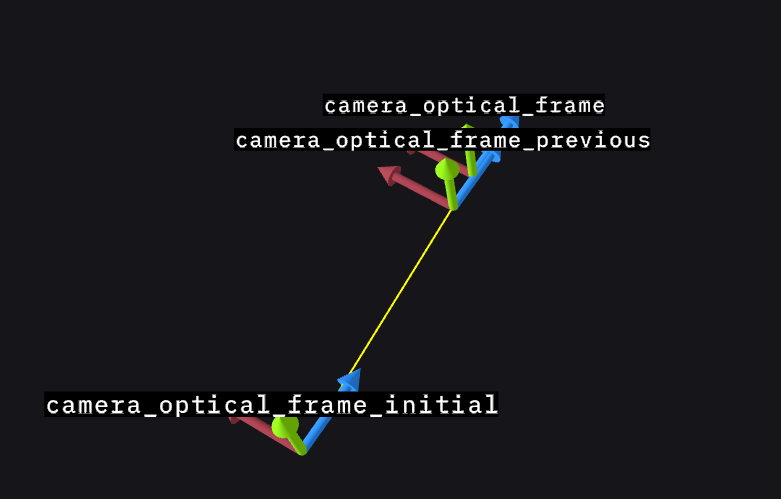
\includegraphics[width=\textwidth]{figures/TF.png}
  \end{minipage}\hfill
  \begin{minipage}{0.5\textwidth}
    \centering
    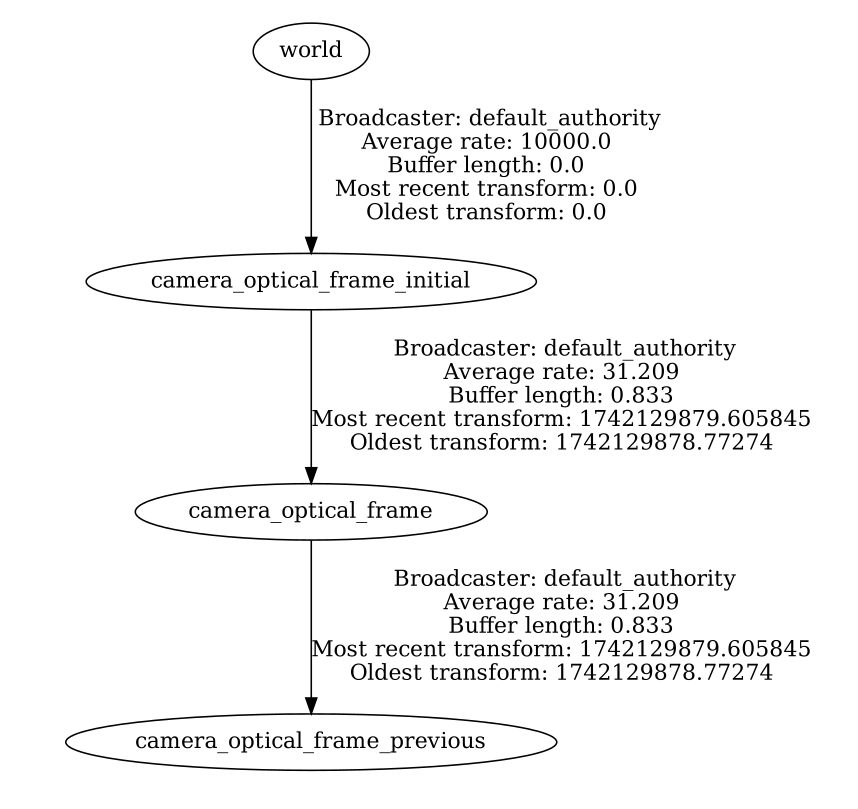
\includegraphics[width=\textwidth]{figures/TF_tree.png}
  \end{minipage}
  \caption{Coordinate frames and ROS2 TF tee. Left: Coordinate frames visualized using Foxglove. Right: ROS2 Transform Tree of the project generated using tf2\_tools. Source: own work} 
  \label{fig:tf}%
\end{figure}%

\subsubsection{Visual odometry algorithm}
\label{sec:OverviewAlgorithm}

The visual odometry algorithm implemented in this work follows a stereo vo and feature-based stereo approach. It
estimates the relative motion of the camera by detecting and matching visual features between
consecutive frames, reconstructing their 3D positions using the depth image, and solving the camera
pose using a Perspective-n-Point (PnP) algorithm~\cite{vo_pnp_survey} with RANSAC for outlier rejection.

A schematic overview of the algorithm steps is presented in Algorithm~\ref{alg:visual_odometry}.

\begin{algorithm}[H]
  \caption{Stereo Visual Odometry Pipeline}
  \label{alg:visual_odometry}
  \begin{algorithmic}[1]
  \Require RGB images $I_{k-1}$, $I_k$, and depth image $D_{k-1}$
  \Ensure Estimated relative pose $(R, t)$ between frames
  \State Detect ORB features in $I_{k-1}$ and $I_k$ using GPU acceleration
  \State Match ORB features between $I_{k-1}$ and $I_k$
  \State Reproject matched keypoints from $I_{k-1}$ into 3D using $D_{k-1}$
  \State Solve PnP with RANSAC using 3D-2D correspondences
  \State Refine the pose estimation with standard solvePnP using inliers
  \State Estimate covariance based on reprojection residuals
  \State Apply statistical filtering and optional exponential smoothing
  \State Output $(R, t)$, covariance matrix, and debug images
\end{algorithmic}
\end{algorithm}

The code of the algorithm is implemented without any ROS2 dependencies, allowing it to be
easily reused in other projects. In the next sections, the main steps of the algorithm are
described in detail.
  
\subsubsection{Feature detection and matching}
\label{sec:FeatureDetectionMatching}

Feature detection and matching constitute the first step in the visual odometry pipeline. In this phase, 
some points, that will serve to compute the desired transformation, will be detected in two consequtive frames.
For this, the ORB (Oriented FAST and Rotated BRIEF) \cite{vo_orb} algorithm will be used.

ORB is a binary feature descriptor that builds upon two classical methods: FAST (Features from
Accelerated Segment Test) \cite{vo_fast} for keypoint detection and BRIEF (Binary Robust Independent Elementary
Features) \cite{vo_brief} for descriptor computation. 

In this context, a keypoint is a point in the image that is distinctive and repeatable (typically corners or blobs), that can be reliably identified across multiple frames.
Around each keypoint, a descriptor is computed: a compact representation of the visual appearance in its local neighborhood. 
These descriptors allow the system to match corresponding features between frames, even under variations in viewpoint.

FAST is a corner keypoint detection algorithm that quickly identifies points in the image with significant intensity
change compared to their surroundings. BRIEF, on the other hand, generates a binary string descriptor
by comparing the intensity of random pairs of pixels in a small patch around the keypoint.

\begin{figure}[H]
  \centering
  \resizebox{0.4\textwidth}{!}{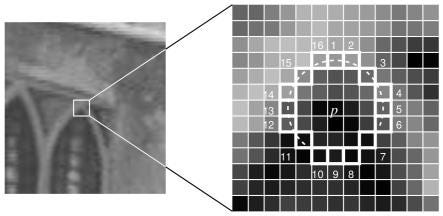
\includegraphics{figures/FAST.jpg}}
  \caption{FAST algorithm. Source: \cite{IntroductionFAST}}
\end{figure}%

ORB enhances these methods by introducing rotation and scale invariance. The orientation of each
keypoint is computed to make BRIEF descriptors rotation-invariant, and a multi-scale pyramid is used
to handle changes in scale. 

The feature extraction and matching process is performed on the GPU using OpenCV's CUDA modules.
This allows real-time processing even at high image resolutions.

The steps involved are:

\begin{enumerate}
  \item Detect ORB features separately in the previous and current grayscale images.
  \item Compute binary descriptors for each detected feature.
  \item Match descriptors between the previous and current frames using brute-force Hamming distance.
  \item Extract the coordinates of matched keypoints for subsequent motion estimation.
\end{enumerate}

\subsubsection{3D-2D correspondences}
\label{sec:3D2DCorrespondences}

Once the feature matching step is completed, the next task is to establish 3D-2D correspondences
between the previous and current frames. This is necessary for estimating the camera motion through
Perspective-n-Point (PnP) techniques.

For each matched keypoint in the previous frame, the corresponding depth value is retrieved from the
depth image associated with that frame. If the depth value is within a valid range, the 2D keypoint is
reprojected into a 3D point using the intrinsic parameters of the stereo camera.

The reprojection follows the standard pinhole camera model:

\begin{equation}
X = (u - c_x) \cdot \frac{d}{f_x}, \quad
Y = (v - c_y) \cdot \frac{d}{f_y}, \quad
Z = d
\end{equation}

where $(u, v)$ are the pixel coordinates of the keypoint, $(c_x, c_y)$ are the coordinates of the principal
point, $(f_x, f_y)$ are the focal lengths in pixels, and $d$ is the depth value.

This process results in a set of valid 3D points extracted from the previous frame, and their corresponding
2D projections detected in the current frame. These 3D-2D pairs are later used to estimate the relative
pose of the camera.

If the depth value is invalid (e.g., missing or outside the valid range), the corresponding match is
discarded to avoid introducing noise into the motion estimation process. In the followign figure, a 
set of detected keypoint can be seen. The ones with valid depth are shown in green, while the ones with invalid depth are shown in red.

\begin{figure}[H]
  \centering
  \resizebox{1.0\textwidth}{!}{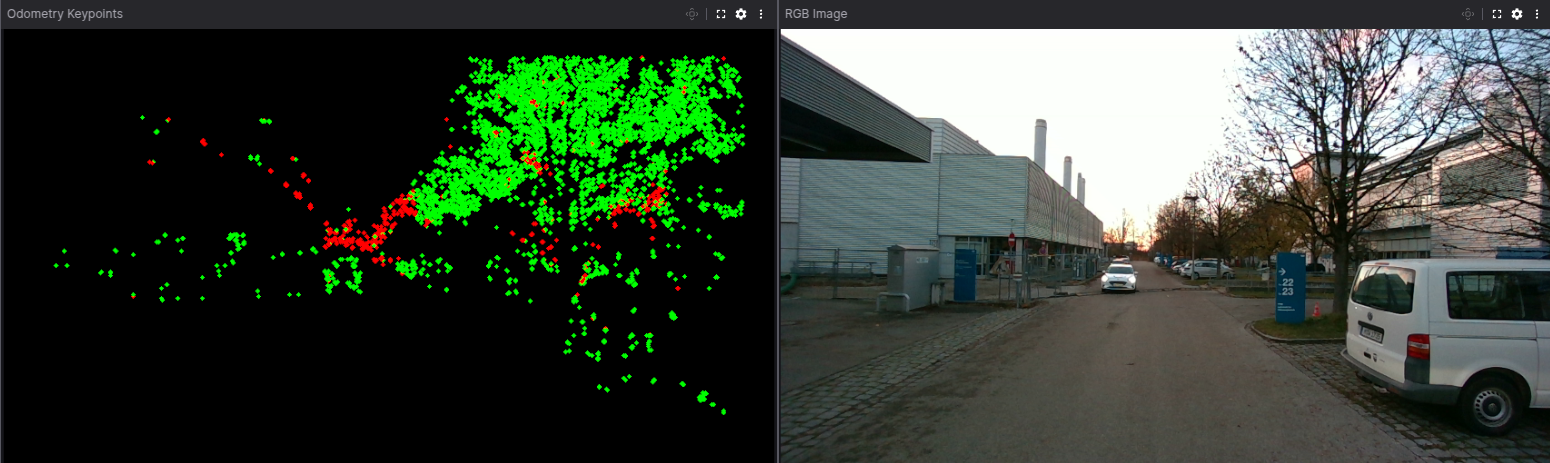
\includegraphics{figures/Keypoints.png}}
  \caption{Odometry Keypoints with depth filtering and RGB Image. Source: own work}
  \label{fig:3D2D_correspondences}
\end{figure}%

\subsubsection{Motion estimation using PnP and RANSAC}
\label{sec:MotionEstimationPnP}

Once 3D-2D correspondences are available, the relative camera motion between two frames can be 
estimated by solving the Perspective-n-Point (PnP) problem~\cite{vo_pnp_survey}. The goal is to compute the rotation 
$\mathbf{R}$ and translation $\mathbf{t}$ that map the 3D points observed in the previous frame to 
their 2D projections in the current image.

\begin{figure}[H]
  \centering
  \resizebox{0.4\textwidth}{!}{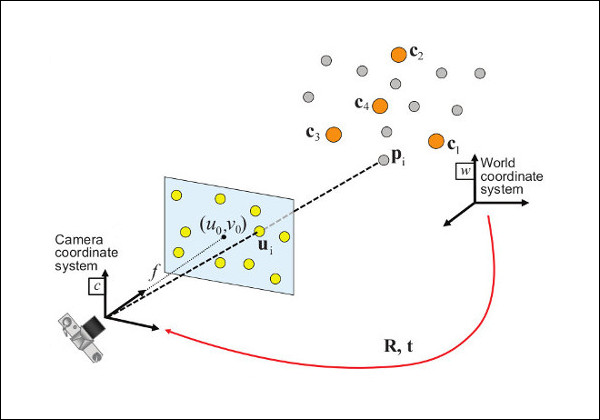
\includegraphics{figures/PnP.jpg}}
  \caption{Perspectective-n-Point (PnP) problem. Source: \cite{vo_pnp_opencv}}
  \label{fig:pnp}
\end{figure}%

Given a set of $n$ correspondences $\{ (\mathbf{X}_i, \mathbf{x}_i) \}$, where $\mathbf{X}_i$ are 3D 
points in the previous frame and $\mathbf{x}_i$ their 2D image projections in the current frame, 
PnP finds a transformation that minimizes the reprojection error under the pinhole camera model:

\begin{equation}
\begin{bmatrix}
u \\ v \\ 1
\end{bmatrix}
\sim
\mathbf{K}
\begin{bmatrix}
\mathbf{R} & \mathbf{t}
\end{bmatrix}
\begin{bmatrix}
X \\ Y \\ Z \\ 1
\end{bmatrix}
\end{equation}

Here, $\mathbf{K}$ is the camera intrinsic matrix, and $\mathbf{R}, \mathbf{t}$ represent the relative 
pose of the current frame with respect to the previous one. The symbol $\sim$ denotes equality up to 
scale in homogeneous coordinates.

In practice, 3D-2D correspondences may include mismatches or noisy observations. To robustly estimate 
the pose in the presence of such outliers, RANSAC (Random Sample Consensus) is used in conjunction 
with PnP.

RANSAC operates by randomly selecting minimal subsets of correspondences, solving the PnP problem for 
each subset, and evaluating how many correspondences agree with the estimated pose. The solution with 
the highest number of inliers is selected, and the pose is then refined using all inliers to minimize 
the overall reprojection error.

In this work, the function \texttt{cv::solvePnPRansac} from OpenCV is used to perform motion estimation. 
This function takes as input the 3D points from the previous frame, their 2D projections in the current 
frame, and the camera intrinsics, and returns the estimated rotation and translation vectors.

The steps involved are:
\begin{enumerate}
  \item Project 3D points from the previous frame into the current image using candidate pose.
  \item Measure the reprojection error against actual 2D keypoints.
  \item Select inliers whose error is below a given threshold.
  \item Repeat for several random subsets and select the best solution.
  \item Refine the pose using all inliers.
\end{enumerate}

The resulting output consists of:
\begin{itemize}
  \item \texttt{rvec} a rotation vector in axis-angle form.
  \item \texttt{tvec} a 3D translation vector.
\end{itemize}

The \texttt{rvec} returned by \texttt{solvePnPRansac} is a Rodrigues rotation vector or axis-angle rotation vector, 
a compact 3×1 representation of rotation. The direction of the vector indicates the axis of rotation, while its 
magnitude represents the rotation angle in radians around that axis. This vector can be converted to a rotation matrix
using the Rodrigues formula.

This matrix describes the transformation from the previous camera frame to the current one, and can 
be used for pose chaining, trajectory estimation, or visual odometry back-end integration.


\subsubsection{Covariance estimation}
\label{sec:CovarianceEstimation}

After estimating the camera pose using PnP and RANSAC, it is often useful to quantify the uncertainty 
associated with this estimate. This is particularly relevant when integrating the pose into filtering 
frameworks, such as an Extended Kalman Filter (EKF), where a covariance is required.

In this work, the pose covariance is approximated based on the reprojection residuals of the inlier 
correspondences identified by RANSAC. Once the best pose has been selected, all 3D points are projected 
onto the image using the estimated transform, and the residual reprojection errors are computed as:

\begin{equation}
\mathbf{e}_i = \mathbf{x}_i^{\text{observed}} - \mathbf{x}_i^{\text{projected}}(R, t)
\end{equation}

The residuals are stacked and used to compute a sample covariance matrix:

\begin{equation}
\Sigma = \frac{1}{N-1} \sum_{i=1}^N (\mathbf{e}_i - \bar{\mathbf{e}})(\mathbf{e}_i - \bar{\mathbf{e}})^T
\end{equation}


Although this approach does not yield an exact pose covariance, it provides a reasonable and fast 
approximation that reflects the quality of the inlier set and the geometric configuration of the 
matched points.


\subsubsection{Motion filtering and smoothing}
\label{sec:MotionFilteringSmoothing}

The pose estimates obtained via PnP are subject to noise due to imperfect keypoint matching, depth
errors, or small instabilities in the feature geometry. To improve the consistency of the estimated
trajectory, a filtering and smoothing step is applied.
Two approaches are combined:
\begin{itemize}
  \item \textbf{Statistical filtering} To detect and remove outliers in both translation and rotation
  components based on deviation from a local history.
  \item \textbf{Exponential smoothing} To smooth the motion estimate over time using a weighted moving
  average.
\end{itemize}

Every component of the translation and rotation vector is  separately. A sliding window is stored for each component to compute its mean and
standard deviation. New values that exceed a fixed threshold or deviate significantly from the mean 
are replaced with the mean.

Once filtered, the values are smoothed using exponential smoothing:

\begin{equation}
s_t = \alpha x_t + (1 - \alpha) s_{t-1}
\end{equation}

where $s_t$ is the smoothed value at time $t$, $x_t$ is the current value, and $\alpha$ is a smoothing
factor between 0 and 1.

Rotation vectors are smoothed component-wise in Rodrigues form. Although this is a simplification
compared to quaternion-based smoothing on $SO(3)$, it performs well in practice for small motions.

After filtering and smoothing, the pose is converted to a 4x4 transformation matrix and stored as the
final motion estimate for the current frame. 


% Translation, rotation, covariance, and debug images.
\subsection{ROS2 Implementation}
\label{sec:ImplementationVisualOdometry}

The previous algorithm was implemented in c++ class called \texttt{VisualOdometry}. This class 
contains all the methods and attributes required to perform the visual odometry algorithm. It
is used in a package called \texttt{visual\_odometry} that performs the ego motion estimation.

The ROS2 node subscribes to the depth image topic, the camera info topic that contains the camera
intrinsic parameters, and the color image topic. It uses the VisualOdometry class to compute the rvec and tvec transformation as 
well as the covariance matrix and the debug image (figure \ref{fig:3D2D_correspondences}).

Once the computation is finished, the node publishes the results on the following topics:
\begin{itemize}
  \item \texttt{/perception\_pipeline/odom} Odometry topic with the camera pose in the camera initial frame.
  \item \texttt{/perception\_pipeline/camera\_frame\_tf} Camera frame transform topic with the camera pose in the previous frame relative to the current frame. It is published as a separate topic because in the Kalman filter steo, this information is required with an exact frame syncronization.
  \item \texttt{/perception\_pipeline/path} Path topic with the camera pose in the world frame (figure \ref{fig:Path}). This topic is used to visualize the camera trajectory.
  \item \texttt{/debug/odometry\_keypoints} Debug topic with the detected keypoint. In red the keypoints with invalid depth and in green the keypoints with valid depth.
  \item \texttt{/tf} The camera frame transform is published as a ROS2 transform. This allows to visualize the camera pose in the world frame using tools like RVIZ or Foxglove.
\end{itemize}

\begin{figure}[H]
  \centering
  \resizebox{0.6\textwidth}{!}{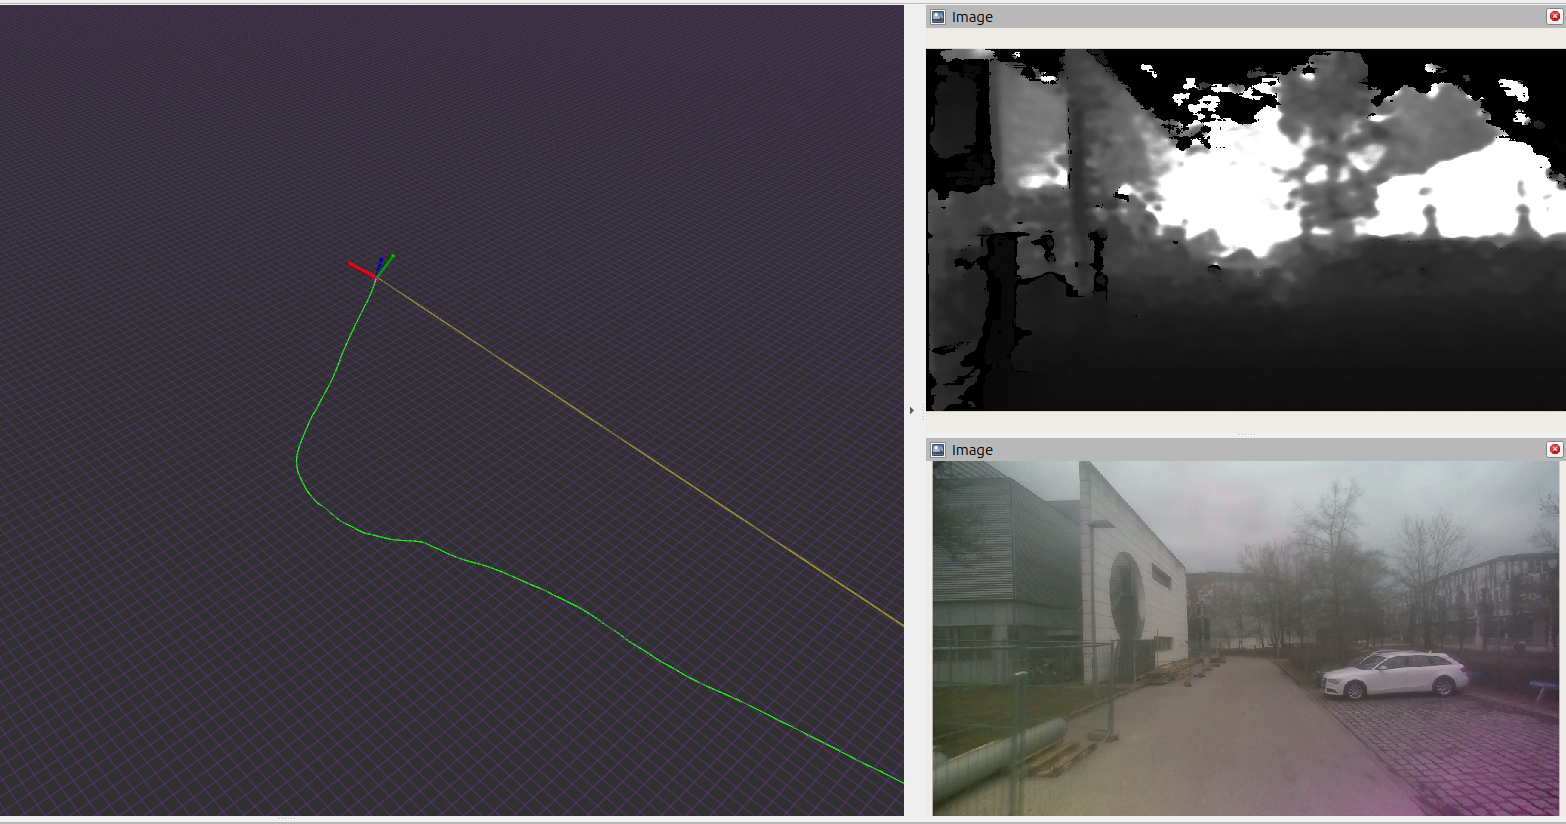
\includegraphics{figures/Path.png}}
  \caption{Path and depth camera topics. Source: own work}
  \label{fig:Path}
\end{figure}%

To configure the node, the following ROS2 parameters were added:

\begin{table}[]
  \centering
  \begin{tabular}{|l|l|}
  \hline
  \textbf{ROS2 Parameter} & \textbf{Definition} \\ \hline
  color\_image\_topic   & Topic name for the input color image. \\ \hline
  depth\_image\_topic   & Topic name for the input depth image. \\ \hline
  camera\_info\_topic   & Topic providing intrinsic camera parameters. \\ \hline
  odometry\_debug\_topic & Topic where debug keypoints for odometry are published. \\ \hline
  camera\_frame\_tf\_topic & Topic containing camera pose as a transform (TF). \\ \hline
  max\_depth\_odom & Maximum valid depth (in meters) used for odometry. \\ \hline
  min\_depth\_odom & Minimum valid depth (in meters) used for odometry. \\ \hline
  odometry\_debug\_image & Enables publishing of debug images with tracked keypoints. \\ \hline
  publish\_odom & Enables publishing of odometry estimates. \\ \hline
  odom\_topic & Topic where odometry data is published. \\ \hline
  publish\_path & Enables publishing of the full trajectory path. \\ \hline
  path\_topic & Topic where the estimated path is published. \\ \hline
  use\_sim\_time & Uses simulation time instead of system time (for Gazebo, etc.). \\ \hline
  \end{tabular}
  \caption{ROS 2 parameters used in visual\_odometry package}
  \label{tab:ros2_vo_params}
\end{table}


\newpage
\section{Perception pipeline: Kalman filter}
\label{sec:KalmanFilter}

After introducing the modules responsible for the depth computation (\ref{sec:StereoImageComputation}), optical flow computation (\ref{sec:OpticalFlowComputation}),
and ego-motion estimation (\ref{sec:EgoMotionEstimation}), this section addresses the core component of the perception 
pipeline: the estimation of a dense six-dimensional field using a Kalman filter. 

The objective of this stage is to compute, for a subset of selected pixels of the image, both their 3D position and 3D
velocity over time. This results in a per-pixel six-dimensional vector that captures the spatial and
dynamic state of the scene.

This idea aligns with the concept of 6D vision (see Section~\ref{sec:6D_Vision}),
which was initially explored at the FTM Chair by Bauer~\cite{previous_tfm_bauer} and later validated in a
ROS1 implementation by Pastor~\cite{previous_tfm_pastor}.

Each point is represented by a \texttt{WorldPoint}, which maintains its own Kalman 
filter and a 6D state vector composed of 3D position and velocity in world coordinates. 
At each timestep, the point’s state is updated using three main sources of input: 

\begin{itemize} 
  \item Optical flow, providing pixel-level motion information between frames. 
  \item Depth data, used to reconstruct the 3D location of the point via reprojection. 
  \item Ego-motion, which accounts for the movement of the camera relative to the environment. 
\end{itemize}




The Kalman filter follows a standard constant-velocity model in 3D space. Predicted states are projected back into 
the image frame for association with new measurements, producing real-time filtered estimates of position and velocity 
at pixel level resolution.

This approach differs from object-based or grid-based tracking by focusing on local, independent point estimation. 
Points are initialized or removed based on visibility, depth consistency, and motion reliability. 
A regular grid helps initialize new points, and the use of OpenMP~\cite{openMP} allows for paralellizing the updates of all active filters
tracked points, leading to a significant speedup in the computation.

The system architecture separates the Kalman logic into a core module that operates independently of ROS, 
and a ROS2 node that manages communication, timing, and visualization. The output includes a 6D image representation, 
debug data, and visualization markers for use in tools such as RViz and Foxglove. 


\subsection{Kalman filter algorithm}
\label{sec:KalmanFilterAlgorithm}

In this module, each selected pixel or \texttt{WorldPoint} is associated with its own Kalman Filter
instance that estimates their local state. The filters operate independently and are updated
at each timestep using new input from the previous perception modules. This approach allows the system 
to maintain a dense spatial resolution while exploit paralell processing capabilities. 

The Kalman Filter, first introduced by R.E. Kalman in 1960~\cite{kalman}, is a recursive 
estimation algorithm, designed for linear, discrete-time dynamical systems with Gaussian noise. 
It estimates the internal state of a system by predicting its evolution over time and correcting
the prediction using new measurements. Taking this into account, the first thing that is necessary 
to implement a Kalman filter is to have the called \textbf{system model} and the \textbf{measurement model}. 

The system model is a state space representation of the system, which describes how the state evolves
over time. It is defined by the following equations:

\begin{equation}
  \mathbf{x}_k = \mathbf{A} \cdot \mathbf{x}_{k-1} + \mathbf{B} \cdot \mathbf{u}_k + \boldsymbol{\omega}_k
\end{equation}

Here, $\mathbf{x}_k$ is the state vector at time $k$, $\mathbf{A}$ is the state transition matrix, 
$\mathbf{u}_k$ is the control input, $\mathbf{B}$ is the control input matrix, and $\boldsymbol{\omega}_k$ 
is the process noise, assumed to be zero-mean Gaussian with covariance $\mathbf{Q}$:

\begin{equation}
  \boldsymbol{\omega}_k \sim \mathcal{N}(\mathbf{0}, \mathbf{Q})
\end{equation}

The measurement model describes how the measurements are related to the state. It is defined by the
following equations:

\begin{equation}
  \mathbf{z}_k = \mathbf{H} \cdot \mathbf{x}_k + \boldsymbol{\nu}_k
\end{equation}

where $\mathbf{z}_k$ is the measurement vector, $\mathbf{H}$ is the measurement matrix, and 
$\boldsymbol{\nu}_k$ is the measurement noise, assumed to be zero-mean Gaussian with covariance 
$\mathbf{R}$:

\begin{equation}
  \boldsymbol{\nu}_k \sim \mathcal{N}(\mathbf{0}, \mathbf{R})
\end{equation}

When both models are linear, as in the equations above, the standard Kalman filter can be used. However, if 
either model is nonlinear, the Extended Kalman Filter (EKF)~\cite{ekf} must be applied. The EKF approximates 
nonlinear functions by linearizing them around the current state estimate using the Jacobian (first order Taylor series approximation).

\subsubsection{Standard Kalman filter}
\label{sec:KalmanFilterClassic}

The standard Kalman filter operates in two main phases at each time step: prediction and correction. Each
phase consists of a sequence of matrix operations that update both the estimated state and its associated
covariance based on the system and measurement models. 

\paragraph{Prediction step}

The prediction step starts by propagating the previous
filtered state $\mathbf{x}_{k-1}$ forward in time using the system model. This results in the predicted state:

\begin{equation}
  \hat{\mathbf{x}}_k = \mathbf{A} \cdot \mathbf{x}_{k-1} + \mathbf{B} \cdot \mathbf{u}_k
\end{equation}

where $\mathbf{A}$ is the state transition matrix, $\mathbf{B}$ the control input matrix, and 
$\mathbf{u}_k$ the control vector at time $k$. The predicted covariance $\hat{\mathbf{P}}_k$ is then computed as:

\begin{equation}
  \hat{\mathbf{P}}_k = \mathbf{A} \cdot \mathbf{P}_{k-1} \cdot \mathbf{A}^\top + \mathbf{Q}
\end{equation}

where $\mathbf{P}_{k-1}$ is the previous covariance and $\mathbf{Q}$ is the process noise covariance. 

\paragraph{Correction step}

Once the state and covariance have been predicted, the correction step begins and the expected measurement is computed using the measurement model:

\begin{equation}
  \hat{\mathbf{z}}_k = \mathbf{H} \cdot \hat{\mathbf{x}}_k
\end{equation}

The predicted measurement covariance is then:

\begin{equation}
  \hat{\mathbf{T}}_k = \mathbf{H}_k \cdot \hat{\mathbf{P}}_k \cdot \mathbf{H}_k^\top
\end{equation}

When a new measurement $\mathbf{z}_k$ is available, it is compared with the predicted measurement 
$\hat{\mathbf{z}}_k = \mathbf{h}(\hat{\mathbf{X}}_{w|k})$ to evaluate how consistent the prediction is 
with the actual observation. The difference between them is known as the innovation vector:

\begin{equation}
  \mathbf{s}_k = \mathbf{z}_k - \hat{\mathbf{z}}_k
\end{equation}

This vector represents the residual between what the filter expected to observe and what was actually measured. 
If the model and previous state are accurate, the innovation should be small and centered around zero. 
Large values in $\mathbf{s}_k$ may indicate unexpected changes in the system or incorrect predictions.

To properly weight the innovation in the update step, its uncertainty must be quantified. This is given by the 
innovation covariance matrix:

\begin{equation}
  \mathbf{S}_k = \hat{\mathbf{T}}_k + \mathbf{T}_k
\end{equation}

Here, $\hat{\mathbf{T}}_k$ is the predicted measurement covariance derived from the current state estimate, and 
$\mathbf{T}_k$ is the measurement noise covariance, defined by the sensor model. The matrix $\mathbf{S}_k$ thus 
quantifies the total expected uncertainty in the innovation vector, combining both predicted state uncertainty 
projected into measurement space and known sensor noise.

The innovation vector and its covariance are crucial for the correction step of the filter: they determine how 
strongly the measurement should influence the state update. A large $\mathbf{S}_k$ implies high uncertainty, 
which results in a smaller correction; conversely, a small $\mathbf{S}_k$ leads to a more aggressive update.

Once the innovation and its covariance are computed, the Kalman gain $\mathbf{K}_k$ is calculated. The Kalman gain
is a matrix that determines how much the predicted state should be adjusted based on the new measurement. It is computed as:

\begin{equation}
  \mathbf{K}_k = \hat{\mathbf{P}}_k \cdot \mathbf{H}^\top \cdot \mathbf{S}_k^{-1}
\end{equation}

Finally, the state and covariance are updated using the Kalman gain and the innovation vector. The updated state
is given by:

\begin{equation}
  \mathbf{x}_k = \hat{\mathbf{x}}_k + \mathbf{K}_k \cdot \mathbf{s}_k
\end{equation}

and the updated covariance becomes:

\begin{equation}
  \mathbf{P}_k = \left( \mathbf{I} - \mathbf{K}_k \cdot \mathbf{H} \right) \cdot \hat{\mathbf{P}}_k
\end{equation}

This completes one full iteration of the standard Kalman filter. The filtered state $\mathbf{x}_k$ and
covariance $\mathbf{P}_k$ serve as the input for the next prediction step.

\subsubsection{Extended Kalman filter}
\label{sec:ExtendedKalmanFilter}

When the system or measurement model is nonlinear, the standard Kalman filter cannot be applied directly.
In such cases, the Extended Kalman Filter (EKF) is used. The EKF extends the classical Kalman filter by
linearizing the nonlinear functions around the current estimate using a first-order Taylor expansion.

Let $\mathbf{f}(\cdot)$ represent the nonlinear system model, and $\mathbf{h}(\cdot)$ the nonlinear measurement
model. The EKF performs the prediction step by applying the nonlinear dynamics to the previous state:

\begin{equation}
  \hat{\mathbf{x}}_k = \mathbf{f}(\mathbf{x}_{k-1}, \mathbf{u}_k)
\end{equation}

The predicted covariance is obtained using the Jacobian $\mathbf{F}_k$ of $\mathbf{f}(\cdot)$ with respect to
the state:

\begin{equation}
  \hat{\mathbf{P}}_k = \mathbf{F}_k \cdot \mathbf{P}_{k-1} \cdot \mathbf{F}_k^\top + \mathbf{Q}
\end{equation}

The predicted measurement is computed by evaluating the nonlinear measurement function:

\begin{equation}
  \hat{\mathbf{z}}_k = \mathbf{h}(\hat{\mathbf{x}}_k)
\end{equation}

and its Jacobian with respect to the state is:

\begin{equation}
  \mathbf{H}_k = \left. \frac{\partial \mathbf{h}(\mathbf{x})}{\partial \mathbf{x}} \right|_{\mathbf{x} = \hat{\mathbf{x}}_k}
\end{equation}

The predicted measurement covariance becomes:

\begin{equation}
  \hat{\mathbf{T}}_k = \mathbf{H}_k \cdot \hat{\mathbf{P}}_k \cdot \mathbf{H}_k^\top
\end{equation}

Given a new measurement $\mathbf{z}_k$, the innovation is:

\begin{equation}
  \mathbf{s}_k = \mathbf{z}_k - \hat{\mathbf{z}}_k
\end{equation}

and the innovation covariance is:

\begin{equation}
  \mathbf{S}_k = \hat{\mathbf{T}}_k + \mathbf{R}
\end{equation}

Once the innovation and its covariance are computed, the Kalman gain is calculated as:

\begin{equation}
  \mathbf{K}_k = \hat{\mathbf{P}}_k \cdot \mathbf{H}_k^\top \cdot \mathbf{S}_k^{-1}
\end{equation}

Finally, the updated state and covariance are:

\begin{align}
  \mathbf{x}_k &= \hat{\mathbf{x}}_k + \mathbf{K}_k \cdot \mathbf{s}_k \\
  \mathbf{P}_k &= \left( \mathbf{I} - \mathbf{K}_k \cdot \mathbf{H}_k \right) \cdot \hat{\mathbf{P}}_k
\end{align}

This completes one full iteration of the Extended Kalman Filter. It retains the recursive structure of the
classical filter while enabling the integration of nonlinear system or measurement models by local
linearization.

\subsection{Mathematical model}
\label{sec:KalmanFilterMathematicalModel}

Now that the Kalman filter algorithm has been introduced, we can define the mathematical model used
in this work. First, the system model is defined and then the measurement model will be defined. 

\subsubsection{System model}

For the system model, the state vector $\mathbf{x}_{k|w}$ is defined as a $6 \times 1$ vector that contains the
position and velocity of the tracked point in world coordinates ($w$):

\begin{equation}
  \mathbf{x}_{k|w} =
  \begin{bmatrix}
    X \\
    Y \\
    Z \\
    \dot{X} \\
    \dot{Y} \\
    \dot{Z}
  \end{bmatrix}
\end{equation}

This vector is propagated over time using a constant-velocity motion model, assuming no acceleration between
frames. When no ego-motion compensation is applied, the evolution of the state is defined by the following 
linear state model system:

\begin{equation}
  \hat{\mathbf{x}}_{k|w} = \mathbf{A}_{k|w} \cdot \mathbf{x}_{k-1|w} + \boldsymbol{\omega}_{k|w}
\end{equation}

where $\hat{\mathbf{x}}_{k|w}$ is the predicted state at time $k$, $\mathbf{A}_{k|w}$ is the transition matrix 
that models constant velocity over the time step $\Delta t$, and $\boldsymbol{\omega}_{k|w}$ is the process noise.

The state transition matrix $\mathbf{A}_{k|w}$ of the system is defined as: 

\begin{equation}
  \mathbf{A}_{k|w} =
  \begin{bmatrix}
    \mathbf{I}_3 & \Delta t \cdot \mathbf{I}_3 \\
    \mathbf{0}_3 & \mathbf{I}_3
  \end{bmatrix}
\end{equation}

where $\Delta t$ is the time elapsed between frames, representing the linear motion model. The process noise is assumed to be zero-mean Gaussian:

\begin{equation}
  \boldsymbol{\omega}_{k|w} \sim \mathcal{N}(\mathbf{0}, \mathbf{Q}_{k|w})
\end{equation}

Where the process noise covariance matrix $\mathbf{Q}_{k|w}$ captures the uncertainty introduced during the 
state prediction. It is derived from the continuous-time system noise model~\cite{6d_vision_detailed} assuming white noise acceleration, 
and discretized using standard integration over the time interval \( \Delta t \). The resulting structure is:

\begin{equation}
  \mathbf{Q}_{k|w} =
  \begin{pmatrix}
    \frac{1}{3} \Delta t^2 \cdot \text{diag}(\sigma^2_{\dot{X}}, \sigma^2_{\dot{Y}}, \sigma^2_{\dot{Z}}) &
    \frac{1}{2} \Delta t \cdot \text{diag}(\sigma^2_{\dot{X}}, \sigma^2_{\dot{Y}}, \sigma^2_{\dot{Z}}) \\
    \frac{1}{2} \Delta t \cdot \text{diag}(\sigma^2_{\dot{X}}, \sigma^2_{\dot{Y}}, \sigma^2_{\dot{Z}}) &
    \text{diag}(\sigma^2_{\dot{X}}, \sigma^2_{\dot{Y}}, \sigma^2_{\dot{Z}})
  \end{pmatrix}
\end{equation}

This formulation assumes that velocity is affected by independent white noise processes in \( X \), \( Y \), and \( Z \), 
and that position integrates this uncertainty over time. As a result, the top-left block of \( \mathbf{Q}_{k|w} \)
corresponds to accumulated uncertainty in position, and the bottom-right to direct uncertainty in velocity.

To introduce the ego-motion compensation, we have to modify the system model. For this we assume, that the WorldPoints are 
transformed with the rotation matrix $\mathbf{R}_k$ and the translation vector $\mathbf{t}_k$, that model the movement of the 
camera between two frames (\ref{sec:MotionEstimationPnP}). The position and velocity components of the state vector $x_k$ are transformed 
as follows:


\begin{equation}
  \begin{bmatrix}
    X \\
    Y \\
    Z \\
  \end{bmatrix}_k
  =
  \mathbf{R}_k
  \cdot
  \begin{bmatrix}
    X \\
    Y \\
    Z \\
  \end{bmatrix}_{k-1|w}
  +
  \begin{bmatrix}
    t_x \\
    t_y \\
    t_z \\
  \end{bmatrix}_k
\end{equation}

\begin{equation}
  \begin{bmatrix}
    \dot{X} \\
    \dot{Y} \\
    \dot{Z} \\
  \end{bmatrix}_k
  =
  \mathbf{R}_k
  \cdot
  \begin{bmatrix}
    \dot{X} \\
    \dot{Y} \\
    \dot{Z} \\
  \end{bmatrix}_{k-1|w}
\end{equation}

which leads to the following updated system state model: 

\begin{equation}
  \mathbf{x}_k = \mathbf{A}_k \cdot \mathbf{x}_{k-1} + \mathbf{u}_k + \boldsymbol{\omega}_k
\end{equation}

Where the individual components are defined as:

\begin{align}
  \mathbf{A}_k &= \mathbf{D}_k \cdot \mathbf{A}_{k|w}, \in \mathbb{R}^{6 \times 6} \\
  \mathbf{D}_k &=
  \begin{bmatrix}
    \mathbf{R}_k & \mathbf{0}_3 \\
    \mathbf{0}_3 & \mathbf{R}_k
  \end{bmatrix}
  \in \mathbb{R}^{6 \times 6} \\
  \mathbf{u}_k &=
  \begin{bmatrix}
    \mathbf{t}_k \\
    \mathbf{0}_3
  \end{bmatrix}
  \in \mathbb{R}^{6 \times 1} \\
  \boldsymbol{\omega}_k &\sim \mathcal{N}(\mathbf{0}, \mathbf{Q}_k)
\end{align}


Now that the ego-motion was introduced in the system model, the covariace matrix $\mathbf{Q}_k$ must be defined. 
This matrix is not only dependant on the process noise $\sigma^2_{\dot{X}}$, $\sigma^2_{\dot{Y}}$, and $\sigma^2_{\dot{Z}}$ like the covarianze matrix
without ego-motion $\mathbf{Q}_{k|w}$, but also on the ego-motion parameters. For this reason a parameter vector containing the ego-motion must be defined. 

In previous works like \cite{6d_vision_detailed}, \cite{previous_tfm_bauer}, and \cite{previous_tfm_pastor}, the ego-motion parameters were defined by the translation 
components and the Euler angles:

\begin{equation}
  \mathbf{p}_k =
  \begin{bmatrix}
    t_{k|x} & t_{k|y} & t_{k|z} & \theta_k & \phi_k & \psi_k
  \end{bmatrix}^T
\end{equation}

This approach has the big disadvantage that the Euler angles are not continuous and can lead to discontinuities in the
covariance matrix. Moreover, its necessary to know beforehand which Euler angle convention was used to build the rotation
matrix $\mathbf{R}_k$. This can lead to confusion and errors in the implementation and also limits the modularity of the code.

For this reason, in this work, the ego-motion rotation components are defined using the Rodrigues vector $\mathbf{r}_k$ that is computed from the rotation matrix $\mathbf{R}_k$:

\begin{equation}
  \mathbf{p}_k =
  \begin{bmatrix}
    t_{k|x} & t_{k|y} & t_{k|z} & r_{k|x} & r_{k|y} & r_{k|z}
  \end{bmatrix}^T
\end{equation}

The Euler-rodrigues vector, as introduced in the chapter \ref{sec:MotionEstimationPnP}, is a continuous representation of the rotation matrix as an vector in $\mathbb{R}^3$ where the length of the vector
is the angle of rotation and the direction of the vector is the axis of rotation \cite{euler_rodrigues_historical,euler_rodrigues} as seen in the figure \ref{fig:rodrigues}.
This representation is continuous and also enables the correct working of the algorithm regardless of how the rotation matrix was computed. 

\begin{figure}[H]
  \centering
  \resizebox{0.30\textwidth}{!}{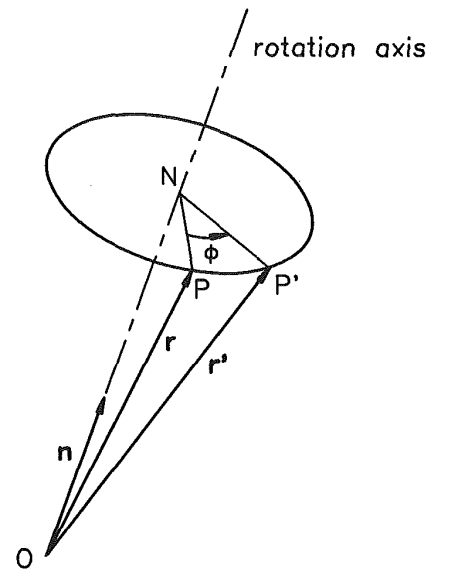
\includegraphics{figures/euler_rodrigues_vector.png}}
  \caption{Rodrigues vector representation of the rotation matrix. Source:~\cite{euler_rodrigues_historical}}
  \label{fig:rodrigues}
\end{figure}

Now that the $p_k$ vector is defined, we can state that the rotation matrix $\mathbf{R}_k$ and the translation vector $\mathbf{t}_k$ are build as follows:

\begin{align}
  \mathbf{R}_k = \mathbf{R}(\mathbf{p}_k + \boldsymbol{\zeta}_k) \\
  \mathbf{t}_k = \mathbf{t}(\mathbf{p}_k + \boldsymbol{\zeta}_k)
\end{align}

Where $\boldsymbol{\zeta}_k$ is the additive white noise of $p_k$ and follows a Gaussian distribution with zero mean and covariance $\mathbf{L}$:

\begin{equation}
  \boldsymbol{\zeta}_k \sim \mathcal{N}(\mathbf{0}, \mathbf{L}), \quad \mathbf{L} = \text{diag}(\sigma^2_{t|x}, \sigma^2_{t|y}, \sigma^2_{t|z}, \sigma^2_{r|x}, \sigma^2_{r|y}, \sigma^2_{r|z}) \in \mathbb{R}^{6 \times 6}
\end{equation}

Taking this into account, the covariance matrix $\mathbf{Q}_k$ is defined as:

\begin{equation}
  \mathbf{Q}_k = \mathbf{D}_k \cdot \mathbf{Q}_{k|w} \cdot \mathbf{D}_k^\top + \mathbf{J}_k \cdot \mathbf{L} \cdot \mathbf{J}_k^\top
\end{equation}

In the previous equation, the term $J_k$ is the Jacobian of the state vector with respect to the ego-motion parameter vector $p_k$:

\begin{equation}
  \mathbf{J}_k = \left. \frac{\partial \mathbf{x}}{\partial \mathbf{p}} \right|_{(\mathbf{x}_{k-1}, \mathbf{p}_k)} \in \mathbb{R}^{6 \times 6}
\end{equation}
  
This Jacobian can be extended as follows:

\begin{equation}
  \mathbf{J}_k = \left. \frac{\partial \mathbf{x}}{\partial \mathbf{p}} \right|_{(\mathbf{x}_{k-1}, \mathbf{p}_k)} =
  \begin{bmatrix}
    \left. \frac{\partial \mathbf{x}}{\partial \mathbf{t}_k} \right|_{(\mathbf{x}_{k-1}, \mathbf{p}_k)} & \left. \frac{\partial \mathbf{x}}{\partial \mathbf{r}_k}  \right|_{(\mathbf{x}_{k-1}, \mathbf{p}_k)} 
  \end{bmatrix}
\end{equation}


The first term, the partial derivative with respect to $\mathbf{t}_k$, corresponds to the direct effect of 
translation on the predicted state. Since the translation vector only affects the position and not the 
velocity, the derivative is:

\begin{equation}
  \frac{\partial \mathbf{x}_{k}}{\partial \mathbf{t}_k} =
  \begin{bmatrix}
    \mathbf{I}_3 \\
    \mathbf{0}_3
  \end{bmatrix}
\end{equation}

The second term, the derivative with respect to the rotation vector $\mathbf{r}_k$, is more complex.
The rotation matrix $\mathbf{R}_k$ is computed from $\mathbf{r}_k$ using the Euler-Rodrigues formula.
In addition to the matrix itself, OpenCV provides the Jacobian 
$\frac{\partial \mathbf{R}_k}{\partial \mathbf{r}_k} \in \mathbb{R}^{9 \times 3}$, which encodes the derivative
of each element of $\mathbf{R}_k$ with respect to the rotation parameters.

Let us denote the intermediate propagated state before ego-motion as:

\begin{equation}
  \mathbf{p}_k = \mathbf{A}_{k|w} \cdot \mathbf{x}_{k-1|w} =
  \begin{bmatrix}
    \mathbf{p}^{\text{pos}}_k \\
    \mathbf{p}^{\text{vel}}_k
  \end{bmatrix}
\end{equation}

where $\mathbf{p}^{\text{pos}}_k$ and $\mathbf{p}^{\text{vel}}_k$ are the position and velocity parts of the
propagated state. Then, the rotated position is given by 
$\mathbf{R}_k \cdot \mathbf{p}^{\text{pos}}_k$, and its derivative with respect to $\mathbf{r}_k$ is:

\begin{equation}
  \frac{\partial (\mathbf{R}_k \cdot \mathbf{p}^{\text{pos}}_k)}{\partial \mathbf{r}_k} = 
  \sum_{i=1}^3 \left( \frac{\partial \mathbf{R}_k}{\partial r_i} \cdot \mathbf{p}^{\text{pos}}_k \right)
\end{equation}

The same procedure applies to the velocity component. The full Jacobian is then:

\begin{equation}
  \frac{\partial \mathbf{x}_{k}}{\partial \mathbf{r}_k} =
  \begin{bmatrix}
    \frac{\partial (\mathbf{R}_k \cdot \mathbf{p}^{\text{pos}}_k)}{\partial \mathbf{r}_k} \\
    \frac{\partial (\mathbf{R}_k \cdot \mathbf{p}^{\text{vel}}_k)}{\partial \mathbf{r}_k}
  \end{bmatrix}
  \in \mathbb{R}^{6 \times 3}
\end{equation}

Combining both components, the full Jacobian with respect to the motion parameters is:

\begin{equation}
  \mathbf{J}_{k|w} =
  \begin{bmatrix}
    \mathbf{I}_3 & \frac{\partial (\mathbf{R}_k \cdot \mathbf{p}^{\text{pos}}_k)}{\partial \mathbf{r}_k} \\
    \mathbf{0}_3 & \frac{\partial (\mathbf{R}_k \cdot \mathbf{p}^{\text{vel}}_k)}{\partial \mathbf{r}_k}
  \end{bmatrix}
\end{equation}


This expression captures how the uncertainty in the ego-motion parameters propagates into the predicted state 
covariance, and allows the filter to adapt to the quality of the visual odometry estimates in a principled way. 
The Jacobian \( \mathbf{J}_k \) is re-evaluated at each time step based on the current predicted state and ego-motion estimate.

Now that the full state prediction model—including ego-motion and its uncertainty—has been defined, we turn our attention 
to the measurement model, which relates the predicted state to the observations available from the stereo camera and 
optical flow pipeline.


\subsubsection{Measurement model}
\label{sec:KalmanFilterMeasurementModel}

The measurement model relates the predicted state to the observed measurements. In this case, the measurements are
obtained from the stereo camera and the optical flow computation. The measurements are defined as a $3 \times 1$ vector:

\begin{equation}
  \mathbf{z}_k =
  \begin{bmatrix}
    u_k \\
    v_k \\
    d_k
  \end{bmatrix}
\end{equation}
where \( u_k \) and \( v_k \) are the pixel coordinates of the tracked point in the image, and \( d_k \) is the depth.
In this project, the depth was considered for the measurment model, instead of the disparity like the previous works,
since most of the modern stereo cameras provide the depth directly as output. 

Unlike the system model, the measurement model is nonlinear. The relationship between the predicted state and the measurements is given by the 
pinhole camera model, which maps the 3D world coordinates to 2D pixel coordinates. The measurement model is defined as:

\begin{equation}
  \mathbf{z}_k = \begin{bmatrix} \mathbf{I}_3 & \mathbf{0}_3 \end{bmatrix} \cdot \frac{1}{w} \cdot \boldsymbol{\Pi} \cdot 
  \begin{pmatrix}
  X \\
  Y \\
  Z \\
  1
  \end{pmatrix}
\end{equation}

where $\boldsymbol{\Pi}$ is the intrinsic projection matrix of the camera, defined as:

\begin{equation}
  \boldsymbol{\Pi} =
  \begin{bmatrix}
    f_x & 0 & c_x & 0 \\
    0 & f_y & c_y & 0 \\
    0 & 0 & 1 & 0
  \end{bmatrix}
\end{equation}

This projection transforms a 3D point in camera coordinates into homogeneous pixel coordinates. The final measured 
pixel location is obtained by normalizing the first two components by the third (perspective division), and taking 
the depth \( Z \) directly from the position vector. Therefore, the nonlinear measurement function 
$\mathbf{h}(\mathbf{x}_{k})$ is defined as:

\begin{equation}
  \mathbf{h}(\mathbf{x}_{k}) =
  \begin{bmatrix}
    \dfrac{f_x X}{Z} + c_x \\
    \dfrac{f_y Y}{Z} + c_y \\
    Z
  \end{bmatrix}
\end{equation}

This maps the predicted 3D point to the expected image coordinates $(u, v)$ and depth \( d = Z \). Since this model 
is nonlinear, the Extended Kalman Filter is used. To apply the correction step of the EKF, the Jacobian of the 
measurement model with respect to the state vector is required.

\begin{equation}
  \mathbf{H}_k = \left. \frac{\partial \mathbf{h}(\mathbf{x})}{\partial \mathbf{x}} \right|_{\mathbf{x} = \hat{\mathbf{x}}_k}
\end{equation}

Only the position part of the state vector affects the measurement, so the Jacobian matrix $\mathbf{H}_k$ has 
non-zero entries only in the first three columns. The matrix $\mathbf{H}_k \in \mathbb{R}^{3 \times 6}$ is computed as:

\begin{equation}
  \mathbf{H}_k =
  \begin{bmatrix}
    \dfrac{f_x}{Z} & 0 & -\dfrac{f_x X}{Z^2} & 0 & 0 & 0 \\
    0 & \dfrac{f_y}{Z} & -\dfrac{f_y Y}{Z^2} & 0 & 0 & 0 \\
    0 & 0 & 1 & 0 & 0 & 0
  \end{bmatrix}
\end{equation}

This Jacobian is evaluated at the predicted state $\hat{\mathbf{x}}_{k}$ and used in the computation of the innovation 
covariance.

\subsection{Implementation}
\label{sec:ImplementationKalmanFilter}

Regarding the implementation of the filter, that will later be used by the corresponding
\texttt{KalmanFilterNode} ROS2 node, it is separated into two main classes as introduces before:

\begin{itemize}
  \item \texttt{WorldPoint}: This class represents a single tracked point in the scene and manages its own Kalman filter.
  \item \texttt{KalmanCore}: This class manages the list of all active filters and handles their initialization and updates.
\end{itemize}

In this subsection, we will describe the high level software architecture of both of them.

\subsubsection{WorldPoint class}
\label{sec:WorldPointClassKalmanFilter}

The \texttt{WorldPoint} class is the core of the Kalman filter implementation. It encapsulates all the logic
for managing a single tracked point in the scene, including its Kalman filter, state prediction,
measurement update, and error code handling. In the following figure \ref{fig:wp} the class diagram of the \texttt{WorldPoint} class is shown.

\begin{figure}[H]
  \centering
  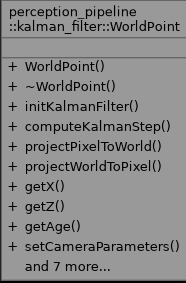
\includegraphics[scale = 0.5]{figures/WorldPoint.png}
  \caption{WorldPoint class. Source: own work} %
  \label{fig:wp}
\end{figure}%

The initialization takes place through the method \texttt{initKalmanFilter()}, which takes a 
pixel location and a depth value, reprojects it to 3D world coordinates, and initializes the 
state vector and covariance. A regular grid ensures that only one point is initialized per 
cell, maintaining a uniform spatial distribution as will be explained in the following section.

The main function for updating each filter is \texttt{computeKalmanStep()}. It takes as input 
the depth image, optical flow, and the current ego-motion estimation. It begins by updating 
the measurement vector using optical flow, then retrieves the new depth from the depth image. 
If the new pixel lies outside the image boundaries or the depth is invalid, the function 
returns an error. Otherwise, it proceeds to the prediction step.

\begin{algorithm}[H]
  \caption{Kalman Filter Step (WorldPoint)}
  \begin{algorithmic}[1]
  \State Get optical flow at previous pixel position
  \State Compute new pixel and read new depth
  \If{new pixel is outside bounds or depth is invalid}
    \State \Return Error
  \EndIf
  \State Predict new state using motion model
  \If{using ego-motion}
    \State Apply rotation and translation
    \State Compute updated uncertainty using Jacobians
  \EndIf
  \State Project predicted state into image
  \State Compute innovation vector and covariance
  \If{3-sigma test fails}
    \State \Return Error
  \EndIf
  \State Compute Kalman gain
  \State Update state and covariance
  \State \Return Success
\end{algorithmic}
\end{algorithm}

If ego-motion compensation is enabled, the predicted state is rotated and translated based on 
the estimated motion of the camera. Additionally, the associated uncertainty is propagated 
using Jacobians of the rotation matrix with respect to the Rodrigues vector. These Jacobians 
are computed using OpenCV, and allow precise propagation of uncertainty due to camera motion.

After predicting the state, the measurement is predicted by projecting the 3D point into the 
image using the pinhole camera model. This expected pixel and depth are then compared to the 
actual measurement, and an innovation vector is calculated. 

Before applying the correction step, a 3-sigma test is used to validate the measurement.
This test ensures that the observed measurement is statistically consistent with the
predicted measurement given the uncertainty. Specifically, it checks whether the Mahalanobis
distance of the innovation vector $\mathbf{s}_k$ is below a threshold:

\begin{equation}
  \mathbf{s}_k^\top \cdot \mathbf{S}_k^{-1} \cdot \mathbf{s}_k < \tau
\end{equation}

where $\mathbf{S}_k$ is the innovation covariance and $\tau$ is the threshold corresponding
to a 99.7\% confidence interval in a chi-squared distribution with 3 degrees of freedom.
If the condition is not met, the measurement is considered an outlier and the correction step
is skipped to maintain filter robustness.


If the update is accepted, the Kalman gain is computed, and the state and covariance are 
updated accordingly. The filter also checks whether the updated 3D point lies within 
acceptable height bounds. If the point is too high or too low, it is discarded.



\subsubsection{KalmanCore class}
\label{sec:KalmanCoreClass}

The \texttt{KalmanCore} class is responsible for managing the full set of active 
\texttt{WorldPoint} filters in the scene. It handles the initialization, update,
removal, and memory management of each tracked point, ensuring a scalable and spatially
uniform filtering process across the image.

\begin{figure}[H]
  \centering
  \includegraphics[scale = 0.5]{figures/KalmanCore.png}
  \caption{KalmanCore class.}
  \label{fig:kalmanCoreClass}
\end{figure}

To guarantee an even distribution of tracked points, a grid-based approach is employed (figure \ref{fig:grid}).
The image plane is divided into a fixed number of rectangular cells, controlled by the
parameters \texttt{grid\_cols} and \texttt{grid\_rows}. Each cell holds at most one
active \texttt{WorldPoint}. This ensures that high-texture regions do not accumulate
redundant points, and low-texture areas are still covered, improving robustness across 
the entire field of view.

\begin{figure}[H]
  \centering
  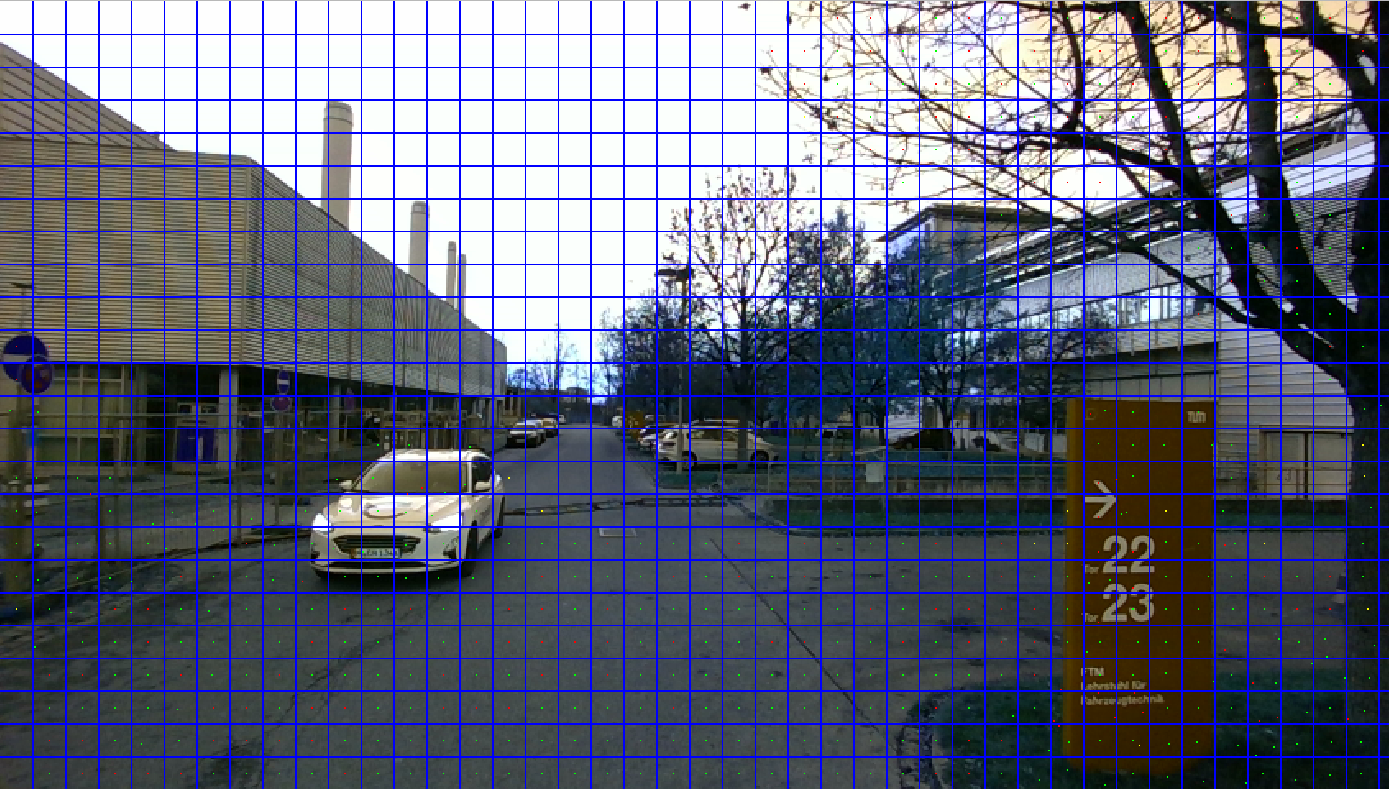
\includegraphics[scale = 0.3]{figures/gridApproach.png}
  \caption{KalmanCore grid.}
  \label{fig:grid}
\end{figure}


The core logic of each frame is executed in the \texttt{updateSyncedData()} method. This
method is responsible for updating all active filters, removing invalid ones, and
reinitializing new points where necessary. The complete process is shown in 
Algorithm~\ref{alg:kalman_core_frame}.

\begin{algorithm}[H]
  \caption{Frame Processing (\texttt{KalmanCore::updateSyncedData})}
  \label{alg:kalman_core_frame}
  \begin{algorithmic}[1]
    \State \textbf{Input:} depth image, optical flow, ego-motion estimate
    \State \textbf{Output:} updated set of WorldPoints
    \ForAll{grid cells $(i,j)$}
      \If{cell has an active WorldPoint}
        \State run \texttt{computeKalmanStep()} for the point
        \If{step fails or point outside bounds}
          \State remove WorldPoint from cell
        \EndIf
      \EndIf
    \EndFor
    \ForAll{empty cells $(i,j)$}
      \State search candidate pixels in image region
      \If{valid depth and point found}
        \State initialize new WorldPoint and store in grid
      \EndIf
    \EndFor
  \end{algorithmic}
\end{algorithm}

The algorithm is divided into two stages. In the first stage, each existing
\texttt{WorldPoint} is updated. If the prediction or correction fails, the point is
discarded. This may occur due to missing depth, invalid image location, or high
innovation error detected by the three-sigma test.

In the second stage, the algorithm checks for empty grid cells. For each unoccupied cell,
a new point is initialized by scanning its corresponding image region for valid pixels
with usable depth. The pixel is reprojected to 3D and passed to \texttt{initKalmanFilter()} 
to start a new filter instance.

The grid ensures that at least one point exists per region at any time, preventing
overlapping estimates and enabling scalable parallel execution. In addition,
the class supports multithreading: the outer loop is parallelized with
OpenMP, allowing all \texttt{WorldPoint}s to be updated simultaneously. This results in
a significant performance gain, especially when tracking hundreds of points across large 
resolutions.

\subsection{ROS2 integration}
\label{sec:ROS2IntegrationKalmanFilter}

The \texttt{KalmanFilterNode} is the central ROS 2 component that connects the Kalman 
filter logic with the perception pipeline. It handles all data flow by subscribing to 
synchronized data input streams, applying the filter update loop, and publishing processed 
outputs and debug information.

The node subscribes to three synchronized input topics: the depth image, the optical 
flow, and the ego-motion transform. Synchronization is performed using 
\texttt{message\_filters::Synchronizer} to guarantee time alignment across all data 
modalities. Accurate synchronization is crucial to prevent inconsistencies in the filter 
prediction and correction steps.

In addition, runtime behavior is fully configurable via ROS 2 parameters. These include the grid 
size, filter parameters such height limits to consider, and whether ego-motion should be used. 
It also allows configuring all relevant noise sources via scalar parameters, 
including the standard deviations of optical flow, depth, process model, and ego-motion 
(rotational and translational) noise. These values are internally used to construct the 
covariance matrices required by the Kalman update equations.

The output of the node is a 2D image encoding the full 6D state field over the image 
plane. This image uses the \texttt{CV\_32FC(7)} encoding, where each pixel contains a 
seven-channel float vector.
\begin{itemize}
  \item Channels 0--2: estimated position \( (X, Y, Z) \)
  \item Channels 3--5: estimated velocity \( (\dot{X}, \dot{Y}, \dot{Z}) \)
  \item Channel 6: binary validity flag (1.0 if valid, 0.0 if empty)
\end{itemize}

For qualitative evaluation and debugging, additional topics are published. 
These include:

\begin{itemize}
  \item A RGB image with the WorldPoint positions overlaid on the original image
  \item A \texttt{MarkerArray} with 3D arrows, representing the estimated velocity field
\end{itemize}

The output of the Kalman Filter is shown in the figure \ref{fig:kalman_output}. 

\begin{figure}[H]
  \centering
  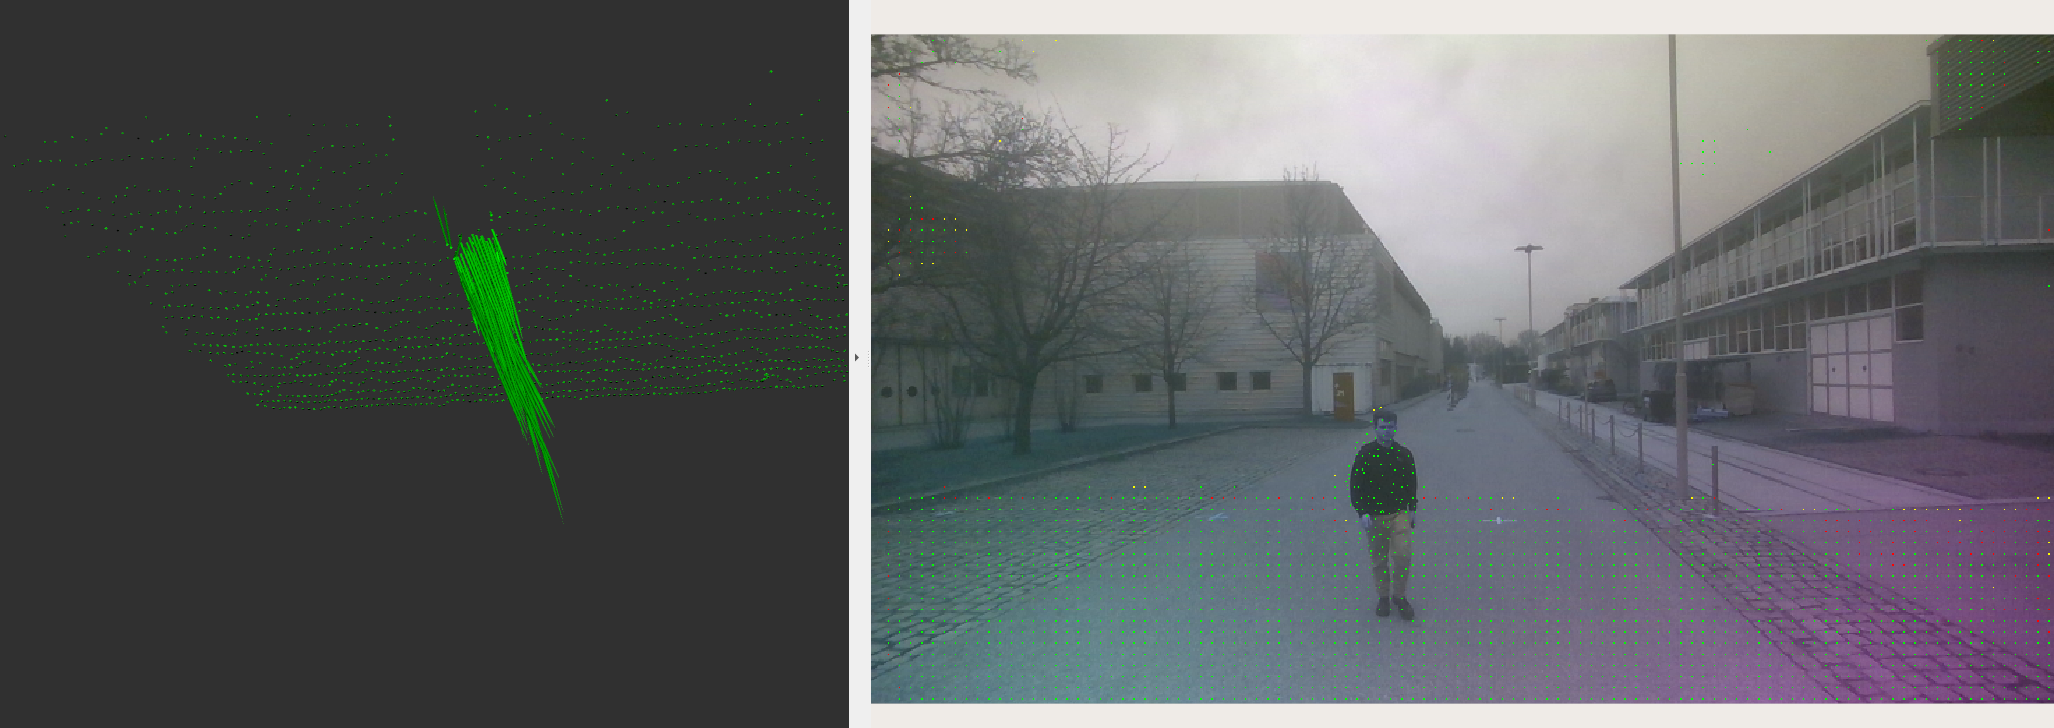
\includegraphics[scale = 0.2]{figures/kalmanOutput.png}
  \caption{Kalman Filter output. Source: own work}
  \label{fig:kalman_output}
\end{figure}

\section{Perception pipeline: Object detection}
\label{sec:PerceptionPipelineObjectDetection}

The final stage of the perception pipeline is the object detection component. It is
responsible for transforming the dense 6D motion field, produced by the Kalman filter,
into a compact set of object-level representations. Each detected object is described by
its spatial extent and estimated velocity, enabling further reasoning in downstream
modules such as criticality assessment.

The object detection component performs two main tasks. First, it filters and selects
reliable motion vectors from the raw state field. Then, it applies a clustering algorithm
to group consistent points into distinct objects. This approach allows the system to
transition from point-based to object-centric perception, which is better suited for
interpreting dynamic scenes.

Like the Kalman filter module, the object detection logic is implemented in a
ROS2-independent source library, and a ROS2 node handles communication and integration
with the rest of the system.

\subsection{Clustering}
\label{sec:Clustering}

The goal of the clustering stage is to aggregate motion vectors into object-level
groups. Each vector, defined by a 3D position and velocity, represents a localized
motion hypothesis estimated by the Kalman filter. Clustering serves to identify sets
of points that likely belong to the same moving object in the environment.

This task is challenging due to the sparsity and variability of the input data.
Objects may vary in size, shape, and velocity; some points may be isolated or
unreliable due to sensor noise or tracking loss. As a result, the clustering method
must be robust, flexible, and capable of handling outliers.

Several clustering techniques have been proposed in literature for similar tasks.
Among the most common are:

\todo{Add references to the clustering algorithms}

\begin{itemize}
  \item \textbf{K-Means~\cite{k_means_original}}: a partition-based algorithm that assigns points to a fixed
        number of clusters. It assumes convex cluster shapes and equal density,
        which is often not the case in real-world perception problems.
  \item \textbf{Hierarchical clustering~\cite{Hierarchical_original}}: a tree-based method that builds a
        cluster hierarchy by recursively merging or splitting groups. It does not
        require prior knowledge of the number of clusters, but has high computational
        cost and is sensitive to noise.
  \item \textbf{Mean Shift~\cite{mean_shift_original}}: a mode-seeking algorithm that clusters based on density
        peaks. It can discover arbitrarily shaped clusters, but tends to be
        computationally expensive and sensitive to bandwidth selection.
  \item \textbf{DBSCAN~\cite{dbscan_original}}: a density-based algorithm that identifies clusters as
        connected regions of high point density. It does not require the number of
        clusters in advance and handles noise explicitly.
\end{itemize}

Given the requirements of this project—unstructured input, unknown number of
objects, and frequent outliers—DBSCAN was selected. It is well suited to segment
point clouds where object boundaries are defined by density rather than geometry.
Moreover, DBSCAN can be extended with a custom distance function, enabling the
integration of both spatial and motion cues into the clustering process.

In this implementation, the algorithm considers two points as neighbors if they
are close in space and exhibit similar velocity vectors. This joint criterion is
more discriminative than position alone, especially in dynamic scenes where
multiple objects may temporarily overlap in 3D space.


\subsection{DBSCAN clustering}
\label{sec:DBSCANClustering}

DBSCAN (Density-Based Spatial Clustering of Applications with Noise) is a
non-parametric clustering algorithm introduced by Ester et al.~\cite{dbscan_original}.
It defines clusters as areas of high point density and treats sparse regions as
separators or noise. This density-based definition allows DBSCAN to discover clusters
of arbitrary shape and to operate without requiring the number of clusters in advance.

The algorithm operates on a dataset of points and requires two parameters:
\begin{itemize}
  \item $\varepsilon$: the neighborhood radius around each point
  \item $minPts$: the minimum number of points within the radius to form a dense region
\end{itemize}

The process begins by iterating over each point in the dataset:
\begin{enumerate}
  \item For a given point, its $\varepsilon$-neighborhood is computed.
  \item If the number of neighbors is greater than or equal to $minPts$, the point is
        marked as a \textit{core point}.
  \item A new cluster is initiated and the neighborhood of the core point is expanded
        recursively to include all density-connected points.
  \item If a point is not a core point and not reachable from any cluster, it is marked
        as noise.
\end{enumerate}

Two points are considered \textit{density-connected} if there exists a chain of core
points such that each is within $\varepsilon$ of the next. This enables clusters to
grow organically around dense regions and stop at natural boundaries.

Figure~\ref{fig:dbscan_clusters} illustrates the basic idea of DBSCAN. Core points have
dense neighborhoods and initiate clusters. Border points lie within the neighborhood
of a core point but lack enough neighbors to be core points themselves. Noise points
do not belong to any cluster.

\begin{figure}[H]
  \centering
  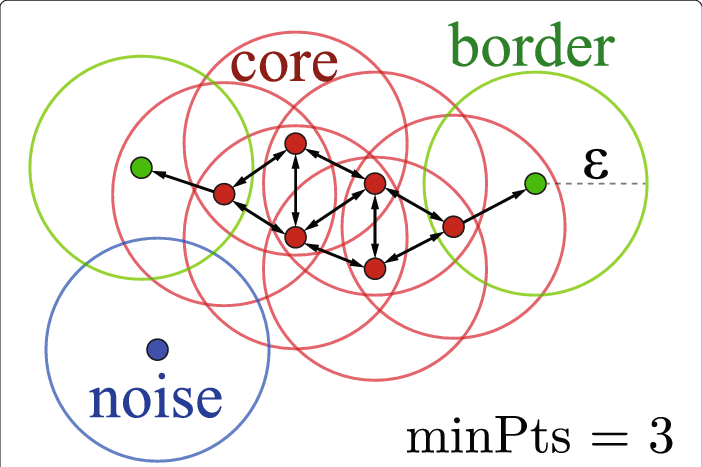
\includegraphics[width=0.45\textwidth]{figures/dbscan_clusters.png}
  \caption{Illustration of DBSCAN clustering: core, border, and noise points. Source:~\cite{dbscan_clusters}}
  \label{fig:dbscan_clusters}
\end{figure}

This structure makes DBSCAN robust to spurious detections and suitable for real-world
scenarios with irregular object shapes. In dynamic environments, it is common for
moving objects to generate clusters of varying density. DBSCAN handles this without
the need to fit a global model or impose strict geometric assumptions.

In our application, the algorithm is applied not in pure Euclidean space, but using a
distance function that incorporates both spatial and motion similarity. The definition
of this distance and its implementation are described in the following sections.

\subsubsection{Implementation}
\label{sec:ObjectDetectionClass}

The \texttt{ObjectDetector} class is the central component responsible for identifying
dynamic objects from the 6D state field computed in the Kalman filter stage. It is
designed as a self-contained module that can be reused and evaluated independently of
the ROS2 framework. The main purpose of this class is to convert a dense field of
motion vectors into a sparse list of detected object representations suitable for
higher-level reasoning.

The class exposes a public method, \texttt{detect()}, which performs the complete
processing pipeline. The input to this method is an OpenCV matrix of type
\texttt{CV\_32FC(7)}, where each pixel encodes a 6D motion estimate and a validity
flag. The output is a list of \texttt{WorldEntity} instances, each corresponding to a
cluster of consistent motion vectors.

Internally, the pipeline consists of three sequential stages. These are described below
in detail.

\paragraph{1. CUDA-based filtering}

The first stage is responsible for identifying valid and informative motion vectors
from the full image. Given that the input may contain a large number of pixels,
including invalid or static ones, it is essential to reduce the dataset before
clustering. To achieve this efficiently, a custom CUDA kernel is used. Each thread in
the kernel processes one pixel, applying a sequence of checks:

\begin{itemize}
  \item Validity: The flag channel must indicate a valid tracked point.
  \item Motion: The magnitude of the velocity vector must exceed a minimum threshold.
  \item Depth: The 3D position must be finite and within a configured spatial range.
\end{itemize}

Points that pass all filters are copied into a device buffer. After kernel execution,
the filtered data is transferred from GPU to CPU memory. This parallel approach allows
processing large images at interactive rates, even when the proportion of valid points
is low.

\paragraph{2. DBSCAN clustering}

The second stage takes the filtered 6D points and performs density-based clustering
using DBSCAN. This is implemented using the \texttt{mlpack} C++ library, which provides
an extensible interface for clustering with custom distance functions. In this case,
a metric combining spatial distance and velocity similarity is used. The motivation
and details of this distance function are presented in the following subsection.

DBSCAN is configured with parameters $\varepsilon$ and $minPts$, which are specified
as ROS parameters. These control the local density required to initiate a cluster and
the radius used to define neighborhoods. Clusters with fewer than the minimum size are
discarded as noise. This helps remove isolated points or spurious detections that may
pass the filtering stage but do not correspond to any coherent object. \paragraph{3. Cluster-to-object conversion}

For each valid cluster found by DBSCAN, a new \texttt{WorldEntity} object is created.
This class encapsulates the aggregate properties of the cluster, including its 3D
bounding box, average velocity, and center position. The conversion is straightforward:
all points in the cluster are passed to the constructor of the \texttt{WorldEntity},
which then computes the relevant statistics. This separation of concerns improves
modularity and simplifies testing.

The high-level flow of the detection pipeline is outlined in
Algorithm~\ref{alg:object_detector_pipeline}.

\begin{algorithm}[H]
  \caption{Object detection pipeline (\texttt{ObjectDetector::detect})}
  \label{alg:object_detector_pipeline}
  \begin{algorithmic}[1]
    \State \textbf{Input:} 6D motion field (OpenCV matrix)
    \State \textbf{Output:} List of \texttt{WorldEntity} objects
    \State
    \State Launch CUDA kernel to extract valid motion vectors
    \State Transfer filtered points from GPU to CPU
    \If{number of valid points $<$ minimum}
      \State \Return empty list
    \EndIf
    \State Instantiate DBSCAN with custom distance function
    \State Run clustering on the filtered point set
    \ForAll{output clusters}
      \If{cluster size $<$ minimum allowed}
        \State discard as noise
      \Else
        \State construct \texttt{WorldEntity} from cluster
      \EndIf
    \EndFor
    \State \Return list of detected entities
  \end{algorithmic}
\end{algorithm}

A structural overview of the class is presented in Figure~\ref{fig:object_detector_uml}.
The figure shows the main attributes, public interface, and key internal methods used
during the detection process.

\begin{figure}[H]
  \centering
  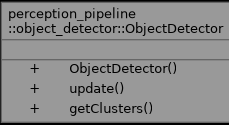
\includegraphics[width=0.6\textwidth]{figures/ObjectDetector.png}
  \caption{UML diagram of the \texttt{ObjectDetector} class. Source: own work}
  \label{fig:object_detector_uml}
\end{figure}

This architecture ensures that the computational workload is kept minimal on the CPU
and that the more expensive filtering operations benefit from parallel execution on
the GPU. The use of \texttt{mlpack} further abstracts the clustering logic, while still
allowing full control over the distance metric and clustering parameters.

The following section describes the custom distance function in detail.


\paragraph{Custom distance function}

The clustering stage uses a custom distance metric that integrates both position and
velocity into the similarity evaluation. This design choice addresses a core limitation
of purely geometric metrics, which may erroneously group objects that are close in space
but move in distinct directions. In dynamic environments, true object boundaries are
often better defined by coherent motion patterns than by absolute position alone.

The distance function is implemented in the \texttt{WeightedPosVelDistance} class
defined in \texttt{point\_distance.hpp}, and used directly within the
\texttt{mlpack::DBSCAN} routine. Each input point is assumed to be a six-dimensional
vector, where the first three components represent the 3D position and the last three
represent the 3D velocity. The distance between two such points, $\mathbf{a}$ and
$\mathbf{b}$, is computed as:

\begin{equation}
  d(\mathbf{a}, \mathbf{b}) = \alpha \cdot \| \mathbf{p}_a - \mathbf{p}_b \|_2 +
                              \beta \cdot \| \mathbf{v}_a - \mathbf{v}_b \|_2
\end{equation}

where $\mathbf{p}_a, \mathbf{p}_b \in \mathbb{R}^3$ are the positions and
$\mathbf{v}_a, \mathbf{v}_b \in \mathbb{R}^3$ are the velocities of the respective
points. The scalar weights $\alpha$ and $\beta$ determine the influence of each term and
can be tuned at runtime via ROS2 parameters. A higher value of $\beta$ increases the
importance of velocity similarity in cluster formation.

The purpose of this formulation is to promote the grouping of points that not only
occupy similar positions in space, but also move with similar direction and magnitude.
This is critical for distinguishing between overlapping or adjacent objects that follow
different trajectories. For example, two pedestrians walking side by side will likely be
clustered together, while one standing still nearby will not be included unless their
motion aligns.

Internally, the \texttt{Evaluate()} method partitions each input vector into position
and velocity components using Armadillo’s \texttt{subvec()} API. The corresponding norms
are computed using \texttt{norm()} and combined with the configured weights to produce
the final scalar value. The function avoids memory allocations and operates efficiently
even on large datasets.

By embedding velocity coherence directly into the clustering distance, this approach
ensures that object-level groupings reflect not only spatial continuity, but also
temporal dynamics. 

\subsubsection{WorldEntity class}
\label{sec:WorldEntityClass}

Each cluster produced by the DBSCAN algorithm is converted into a \texttt{WorldEntity}
object, which encapsulates its geometric and kinematic properties in a compact
representation. The class is initialized with a list of 3D points and corresponding
velocity vectors, from which it computes the centroid, average velocity, and an
oriented bounding box. These quantities are stored internally and accessed via public
getter methods. The centroid is computed as the arithmetic mean of all 3D positions,
and the average velocity is calculated analogously from the velocity vectors. These two
features provide a representative location and motion estimate for the object.

The bounding box is computed using a Principal Component Analysis (PCA), which enables
an orientation-aware description of the cluster's shape. The procedure consists of the
following steps:

\begin{enumerate}
  \item Center the input data by subtracting the mean position from each point.
  \item Form a \( 3 \times N \) matrix containing all centered 3D points.
  \item Compute the covariance matrix of the centered data.
  \item Solve the eigenvalue decomposition to obtain three orthogonal basis vectors.
  \item Project all points into this PCA-aligned coordinate system.
  \item Determine the minimum and maximum bounds along each principal axis.
  \item Reconstruct the eight corners of the bounding box in world coordinates by
        transforming the axis-aligned box in PCA space back to the original frame.
\end{enumerate}

This results in an oriented bounding box that tightly encloses the cluster. The three
axes of the box correspond to the directions of maximum variance in the data, and the
box dimensions reflect the spatial spread along those axes. If the number of points is
too low to perform PCA reliably, a fallback axis-aligned bounding box is computed
directly from the minimum and maximum values in each coordinate dimension.

This bounding box serves not only as a geometric representation of the object, but also for the 
computation of the criticallity metric. Thanks to the bounding boxes, its not necessary anymore
to assume the objects to be point-like, but they can be represented as 3D boxes. This allows for a more accurate

In addition to geometric information, the class assigns a unique identifier to each
entity and includes utility methods for converting its contents into ROS-compatible
messages. These include a method for generating a visualization marker and another for
publishing the entity as part of a message array. The class diagram shown in
Figure~\ref{fig:world_entity_uml} summarizes the internal structure and public
interface of the implementation.

\begin{figure}[H]
  \centering
  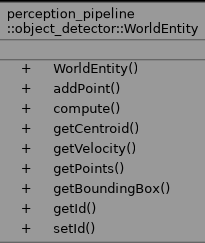
\includegraphics[width=0.5\textwidth]{figures/WorldEntity.png}
  \caption{UML diagram of the \texttt{WorldEntity} class. Source: own work}
  \label{fig:world_entity_uml}
\end{figure}

This class provides a consistent abstraction between the clustering algorithm and the
next stages of the perception pipeline, enabling object-level reasoning based on motion
vector fields.


\subsubsection{ROS2 integration}
\label{sec:ROS2IntegrationObjectDetection}

The \texttt{ObjectDetectorNode} serves as the ROS2 interface to the object detection
module. It connects the independent detection logic with the rest of the perception
pipeline and is responsible for receiving motion data, triggering clustering, and
publishing object-level representations. The node subscribes to a single topic
containing the 6D motion field output from the Kalman filter stage. This field is
published as a \texttt{sensor\_msgs::msg::Image} message with encoding
\texttt{CV\_32FC(7)}. Each pixel in the image stores a seven-dimensional float vector:
three values for position, three for velocity, and one flag indicating if the data is
valid.

Upon receiving a new message, the callback function \texttt{callback6dImage()} converts
the input to a \texttt{cv::Mat}, which is then passed to the detector. The
\texttt{ObjectDetector} instance processes the image and returns a list of clustered
entities. These clusters are then published in two forms: as RViz visualization markers
and as structured messages for downstream consumption.

The structured output is published on the \texttt{/object\_clusters} topic using a
custom message type \texttt{ClusteredObjectArray}. This message encapsulates all
detected objects for a given frame. It contains a header, the number of clusters, and a
vector of \texttt{ClusteredObject} messages. Each \texttt{ClusteredObject} includes:

\begin{itemize}
  \item \texttt{id}: a unique integer identifier for the object
  \item \texttt{position}: a \texttt{geometry\_msgs::Point} representing the centroid
  \item \texttt{velocity}: a \texttt{geometry\_msgs::Vector3} with average motion
  \item \texttt{bb\_marker}: a \texttt{visualization\_msgs::Marker} for RViz
  \item \texttt{bounding\_box}: a custom message of type \texttt{BoundingBox}
\end{itemize}

The \texttt{BoundingBox} message defines the geometry of the oriented bounding box as a
list of eight 3D corners, stored as an array of \texttt{geometry\_msgs::Point}. This
explicit representation of the box enables further geometric reasoning in later stages
of the pipeline, including volume checks, trajectory prediction, or collision
assessment.

In parallel to structured outputs, the node publishes markers for visualization. These
include the bounding box as a wireframe, the motion vector as an arrow, and the
clustered points as spheres, all in the \texttt{camera\_optical\_frame}. This visual
feedback is critical for debugging and validation, and is useful during live operation
as well as during dataset annotation or offline replay.

All relevant parameters of the node are loaded from the ROS2 parameter server. These
include the clustering radius $\varepsilon$, the minimum number of points
\texttt{minPts}, velocity threshold, and the weights \texttt{pos\_weight} and
\texttt{vel\_weight} for the custom distance metric. The input and output topics can
also be configured via parameters to ensure compatibility with different integration
setups.

The node follows standard ROS2 design conventions and uses
\texttt{message\_filters::Synchronizer} when required to align incoming data. The
internals of the clustering remain decoupled from ROS, ensuring that the core
algorithm remains portable and testable in isolation.

With this structure, the object detection node forms a robust interface layer that
bridges raw motion estimation with object-level perception, providing consistent,
interpretable outputs for higher-level modules such as criticallity estimation,
trajectory planning, or logging and evaluation tools.



\section{Criticallity pipeline: TTC computation}
\label{sec:CriticallityPipelineTTCComputation}

% Explain different critically metrics

% ====================================================================
% ================== Experiments and Results =========================
% ====================================================================
\chapter{Experiments and Results}
\label{chap:ExperimentsAndResults}

% - Introduction to the chapter
% - Explain how the experiments were conducted
% - Explain how the results were evaluated

\section{Camera hardware selection}
\label{sec:CameraHardwareSelection}

% - Explain how the camera was selected

\section{Experimental setup}
\label{sec:ExperimentalSetup}

% - Explain how the experiments were conducted

\section{Perception pipeline evaluation}
\label{sec:PerceptionPipelineEvaluation}

\subsection{Stereo image computation}
\label{sec:StereoImageComputation}

% - Explain how the stereo image computation was evaluated
\subsection{Optical flow computation}
\label{sec:OpticalFlowComputation}
% - Explain how the optical flow computation was evaluated

\subsection{Ego motion estimation}
\label{sec:EgoMotionEstimation}  
% - Explain how the ego motion estimation was evaluated

\subsection{Kalman filter}
\label{sec:KalmanFilterEvaluation}
% - Explain how the Kalman filter was evaluated

\subsection{Object detection}
\label{sec:ObjectDetectionEvaluation}
% - Explain how the object detection was evaluated

\section{Criticallity pipeline evaluation}
\label{sec:CriticallityPipelineEvaluation}


% ====================================================================
% ================== Discussion ======================================
% ====================================================================
\chapter{Summary and Conclusion}
\label{chap:SummaryAndConclusion}- High level explanation on how the work will be structured. 
- What the perception and criticallity pipeline are
- Go through each component. 